\documentclass{report}

\usepackage{titletoc}
\usepackage{parskip}
\usepackage{graphicx}
\usepackage{verbatim}
\usepackage{fontspec}
\usepackage{minted}

% Main font set so symbols display outside code blocks. You may not need this
\setmainfont[Ligatures=TeX]{Linux Libertine O}

% This font supports all logic symbols in monospace as far as I can tell. You may need to install
\setmonofont{DejaVu Sans Mono}

\graphicspath{ {/home/anna/workspace/EquivalencesApp/report/i/} }

\makeatletter
\def\@makechapterhead#1{%
  \vspace*{50\p@}%
  {\parindent \z@ \raggedright \normalfont
    \interlinepenalty\@M
    \Huge \bfseries #1\par\nobreak
    \vskip 40\p@
  }}
  \makeatother

\begin{document}
% This line removes red boxes from "incorrect syntax". Needs to be NOT in the pre-amble
\expandafter\def\csname PY@tok@err\endcsname{}

\title{Equivalence Teaching Tool}
\author{Anna Thomas}

\maketitle

\tableofcontents

\chapter{Introduction}

\section{Motivation}

All logics are based on propositional logic in some form, so it is important that new students learn how to use it. Propositional logic consists of syntax, semantics and proof theory; syntax is the formal language which is used to express concepts, semantics provide meaning for the language and proof theory provides a way to convert one formula into another using a defined set of rules.

We know that new students learning propositional logic can struggle to understand the rules and how they should be applied to formulae. To help with this our idea is to create an equivalence teaching tool; this will be a tablet application which will allow a user to apply rules to a formula until they have reached the desired equivalence.

\section{Approach}

We decided early on in the project that the tool should be an Android tablet application as opposed to a web or mobile one; this allows for an intuitive, interactive design while still having a large screen space.

The tool can be divided up into its main component parts: the parser, tree constructor, tree processing and tablet interface. The parser will be generated by the ANTLR4 parser generator, the tree constructor, processing code and the tablet interface will be written in Java with the interface using the Android SDK.

The parser requires a grammar to generate the relevant parser components. This will be used to parse the initial equivalence and return the ANTLR4 tree representation of the string.

The tree constructor is required to take the ANTLR4 representation of a tree and convert it into a more useful data structure which can be modified and displayed easily. The operators and atoms of the formula will be represented as nodes and leaves respectively.

Tree processing will be used to internally calculate which rules are applicable to each node and will allow us to subsequently manipulate the tree by applying these rules.

The interface will have an intuitive design displaying the current formula's formation tree (generated by the tree constructor) and allowing a user to click on the operators to apply a rule.


\section{Objectives}

The application should have some key features. These are outlined below:

\begin{enumerate}
\item Graphical tree representation of formulae

Representing the formula as a tree structure allows a user to see exactly how the formula should be read and can help them understand the order of operations. It also allows the user to click on an operator to select a rule for it; this is much more intuitive than just clicking on the whole formula and not knowing which section the rule would be applied to.

\item Undo/Redo functionality

Previous equivalent formulae will be displayed above the current formula. When an old formula is selected it will expand into tree form and the formulae below it are faded out \textit{(Undo)}. This will allow a user to perform rules on the old tree or select one of the later faded trees \textit{(Redo)}. When a rule is applied, the faded formulae will be removed from the history allowing the user to continue on from that point (Figure \ref{undo}).

\begin{figure}[ht]
    \centering
    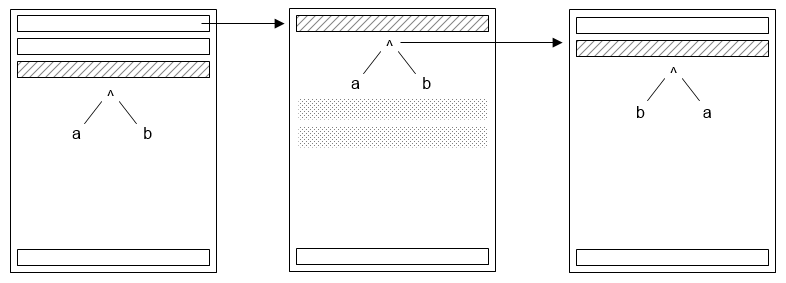
\includegraphics[width=\textwidth]{undo.png}
    \caption{Undo functionality - Clicking a previous equivalence shows the formula tree for that equivalence and sets the undone history as translucent. Applying a rule then overwrites the undone history.}
    \label{undo}
\end{figure}

\item Generated equivalences

We want to allow the user to have equivalences automatically generated for them to solve. This would be implemented by running the tool on a generated formula to give a significantly different equivalent one. The key advantage of having this feature as well as allowing manual entry of equivalences would be that the user will have a continuous supply of new equivalent logic formulae after completing all those set by their lecturer. This also requires generating the initial formula for the tool to be run upon or allowing the user to manually enter the first formula and have the second one generated for them.

\item Difficulty setting

Extending the idea of generated equivalences, we could allow the user to select a difficulty. This would be calculated by the length of the generated formula and how many rules were applied to get its equivalent formula. We could also provide a recommended difficulty based on how many previous equivalences they have completed and how far from optimal their solutions were.

\item Help

Providing the user with help is key to their improvement. Once an equivalence has been set up, the tool should calculate the optimal route from the starting formula to the desired end point. Upon finishing the equivalence the user will receive a message telling them how far from the optimal solution they were and give them the option to try again or to view the optimal solution. Throughout there will also be a help button available that will suggest the next step to the user on request; this includes the recommendation to undo certain steps if the user reaches a cycle. Pointing out mistakes could also be enabled, so if the user has completed a cycle or is heading towards a dead end they will be prompted to consider a different strategy.

\end{enumerate}

\section{Achievements}

%What is the problem, why is it interesting and what’s your main idea for solving it?

We have been challenged with developing an android application to help new students learn propositional logic and to complete logical equivalences. In this section we will discuss our motivation, approach and objectives.

\chapter{Logic}

We are assuming a basic understanding of propositional logic, including the operators and rules that are defined in the system. For more information on these please visit the Wikipedia article\cite{propositionalwiki}.

\section{Propositional Logic}

Propositional logic is a branch of logic that studies ways of combining and modifying whole sentences, statements or propositions to form more complex propositions. It is a formal system containing logical relations and properties which are derived from these methods of joining or altering statements.

A logical system contains three major parts:

\begin{enumerate}
\item Syntax - the formal language that is used to express concepts.
\item Semantics - provide meaning for the language.
\item Proof theory - provides a way to convert one formula into another using a defined set of rules.
\end{enumerate}

Logical definitions:

\begin{itemize}
\item \emph{Atomic} - A formula whose logical form is $\top$, $\bot$ or \textit{p} for an atom \textit{p}.
\item \emph{Negated atomic} - A formula of the form $\neg$\textit{p}.
\item \emph{Negated formula} - A formula of the form $\neg$\textit{A} for a formula \textit{A}.
\item \emph{Conjunction} - A formula of the form \textit{A}$\land$\textit{B}.
\item \emph{Disjunction} - A formula of the form \textit{A}$\lor$\textit{B}.
\item \emph{Implication} - A formula of the form \textit{A}$\to$\textit{B}, where \textit{A} is the \emph{antecedent} and \textit{B} is the \emph{consequent}.
\item \emph{Literal} - A formula that is either atomic or negated atomic.
\item \emph{Clause} - A disjunction of one or more literals.
\end{itemize}

A \textit{statement} is defined as a meaningful declarative sentence that is either true or false. For example, a statement could be: 

\begin{itemize}
\item `Socrates is a man.'
\item `All men live on Earth.'
\end{itemize}
A statement can be constructed of multiple parts, for example, the above statements can be combined into:

\begin{itemize}
\item `Socrates is a man and all men live on Earth.'
\end{itemize}
Each part of this statement can be considered a proposition. Propositional logic involves studying the connectives that join these such as \textit{`and'} and \textit{`or'} (to form conjunctions and disjunctions), the rules that determine the truth values of the propositions and what that means for the validity of the statement.

\section{First Order Logic}

\section{Truth tables}
\label{sec:truth_tables}

It is necessary to understand the meanings of the symbols used in a language. Truth tables are mathematical tables used in logic to compute the functional values of logical expressions. They can be used to determine whether or not a propositional logic statement is logically valid.

A \textit{situation} determines whether each propositional atom is true or false. A truth table shows all the situations the input variables can be in. We write 1 for true and 0 for false as shown below:

\vspace{5 mm}
\begin{center}
  \begin{tabular}{ || c | c || c | c || }
    \hline
    A & B & A$\land$B & A$\lor$B \\ \hline
    1 & 1 & 1 & 1 \\
    1 & 0 & 0 & 1\\
    0 & 1 & 0 & 1 \\
    0 & 0 & 0 & 0 \\
    \hline
  \end{tabular}
\end{center}
\vspace{5 mm}

Truth tables can be used to define any operators, including any new ones which might be desired.

\chapter{Related Work}
\label{chap:related_work}

\section{Logic Daemon}

Created in Texas A\&M University, the Logic Daemon\cite{logicdaemon} is an online logic proof checker. It comprises a simple web page with two small text input boxes for the premises and conclusion and then one large text box for applying primitive rules (Figure: \ref{logicdaemon}).

While this tool does allow us to apply rules to prove equivalences we do not find it very intuitive to use at all. The interface itself looks quite unclear and isn't user friendly so it would not be suited to new students. Applying the rules to the premises is also quite confusing as it shows all the rules and does not alert the user to the fact they cannot be applied until they have already clicked on it. We found this a frustrating way of attempting a proof; as such, we intend to only display the rules that can be applied in the current situation.

However, it is a useful tool for those more knowledgeable about logic for checking proofs once they have got to grips with the interface. It also has a \textit{`Get Help'} button to suggest which rule to use next. We hope to use the idea of a help button in our project but to build upon it in order to provide more extensive help such as showing when an action has been repeated (i.e. a cycle has been reached).

We hope that our tool will be more intuitive to use because we will display formulae as formation trees with interactive nodes to apply rules with. This should provide a more straight forward way of presenting the rules to new students.

The website also provides a simple equivalence checker, well-formed formula checker and countermodel checker. These are all similar tools useful in logic but again the interface is not particularly intuitive or user friendly.

The Logic Daemon tool also provides support for first order logic which we are not planning on covering in our main tool. However, this could be implemented as an extension at the end of our project.

\begin{figure}[ht]
    \centering
    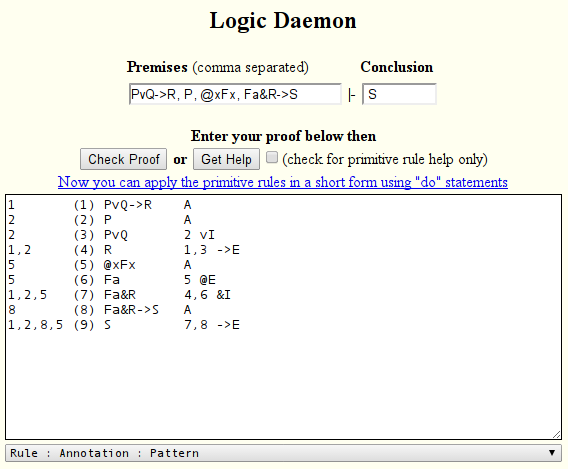
\includegraphics[width=\textwidth]{logicdaemon.png}
    \caption{Logic Daemon}
    \label{logicdaemon}
\end{figure}

\section{Pandora}
\label{sec:pandora}

Pandora\cite{pandora} is a tool created by Imperial College London; it stands for `Proof Assistant for Natural Deduction using Organised Rectangular Areas'. It can be used to prove that a goal formula follows from the given formulae. Pandora allows the user to repeatedly apply natural deduction rules (Figure: \ref{pandora}).

We do not intend to include natural deduction in our tool as we want to focus more on solving propositional logic equivalences. Pandora is a much nicer tool than the Logic Daemon and we find it much more intuitive and easy to use.

Pandora allows a user to apply rules forwards or backwards. We know from using Pandora that some proofs are easier to complete working backwards; as such, this is an idea we hope to incorporate into our tool by allowing the user to expand either the top or bottom formula to show its formation tree and to apply rules. 

\begin{figure}[ht]
    \centering
    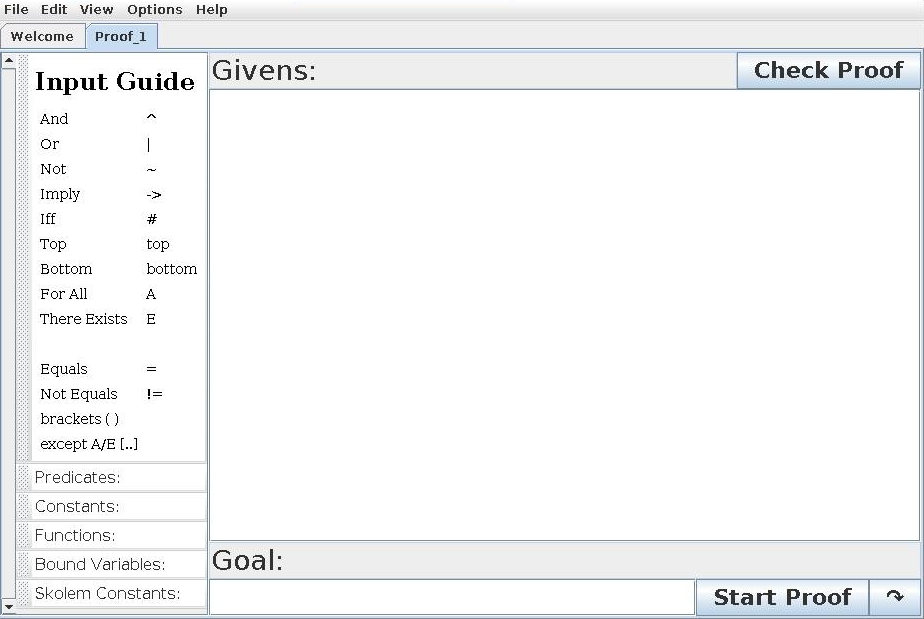
\includegraphics[width=\textwidth]{pandora.jpg}
    \caption{Pandora}
    \label{pandora}
\end{figure}

\section{Logic Solver}

This is an Android application to show truth tables and possible logical equivalences. It looks like it has been made as a phone application as on a tablet it fills very little of the screen and it is difficult to click on some of the links (Figure \ref{logicsolver}).

The user can apply rules to the formula they enter into the application; this is done by selecting the rule they want out of a list which is then applied to the formula. However they cannot use this application to solve an equivalence as they can only enter one formula and then apply rules to that. We want to improve upon this in our own application by allowing the user to enter two formulae and work from either end to solve it.

The list of rules that is offered to the user only shows the rules that can be applied to the current formula. We want to also offer this behaviour as there are far too many rules to display them all to the user and expect them to sort through which could be applied.

Formulae are displayed simply in the application; we think this could be improved upon and want to display our current formula as its formation tree.

\begin{figure}[ht]
    \centering
    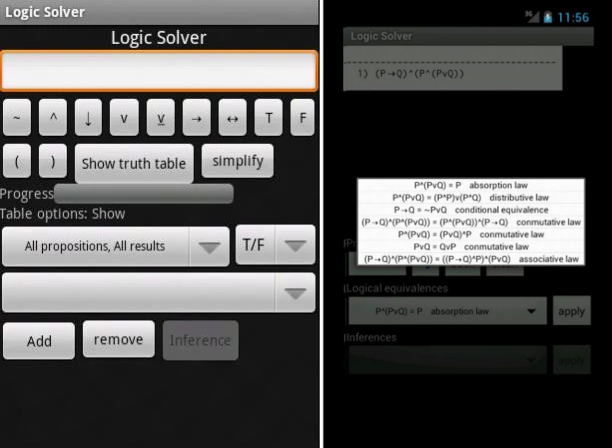
\includegraphics[width=\textwidth]{logicsolver.png}
    \caption{Logic Solver Android Application}
    \label{logicsolver}
\end{figure}

\section{Truth Tables}

Truth Tables is also an Android application mainly for use on a phone. It simply generates and displays truth tables based on a logical formula (Figure \ref{truthtables}).

We currently do not plan on adding truth tables to our application as we do not believe it is as useful for learning and understanding propositional logic as our other ideas. However, this could be added as an extension at the end of the project depending on how much time is left.

\begin{figure}[ht]
    \centering
    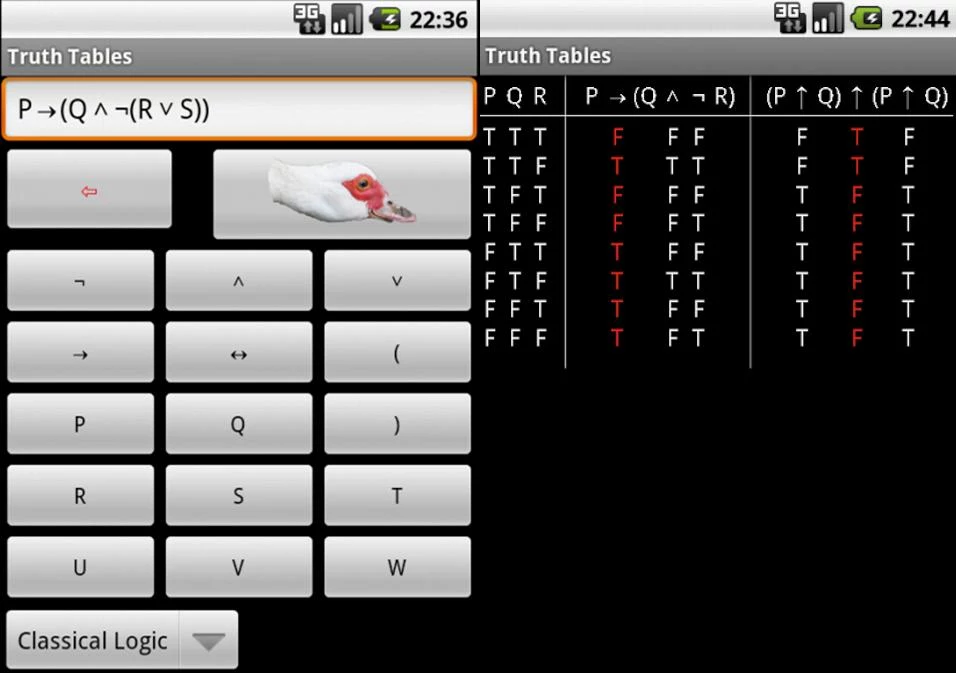
\includegraphics[width=\textwidth]{truthtables.png}
    \caption{Truth Tables Android Application}
    \label{truthtables}
\end{figure}

\section{LogicCalc}

LogicCalc is an Android application for solving problems with propositional logic. It allows the user to create workbooks to save and print their proofs (Figure \ref{logiccalcapp}). However we had trouble running it on our Nexus tablet.

We like the idea of saving proofs in workbooks for future reference. This is something we had not considered before and are curious to explore as an extension. This functionality would be useful for students completing exercises that needed a paper hand in as they would be able to save and print them off.

\begin{figure}[ht]
    \centering
    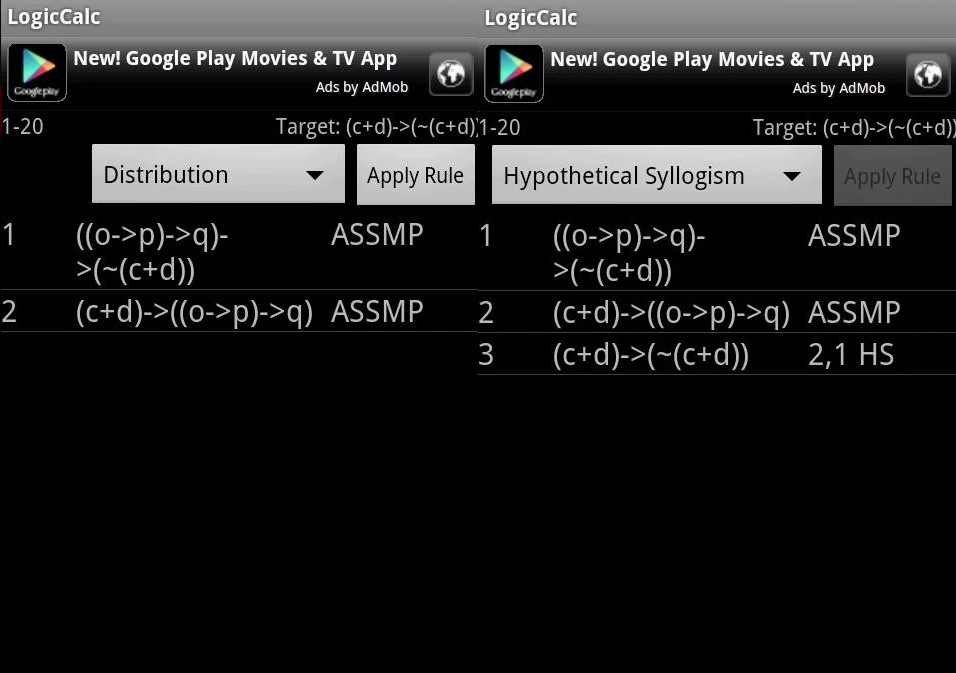
\includegraphics[width=\textwidth]{logiccalcapp.png}
    \caption{LogicCalc Android Application}
    \label{logiccalcapp}
\end{figure}

\section{Propositional Logic Calculator}

The Propositional Logic Calculator\cite{logiccalc} finds all of the models of a given propositional formula. The website tells us that the only limitation for this calculator is that we have only three atomic propositions to choose from: p,q and r (Figure: \ref{logiccalc}).

Propositions are entered using the keyboard they provide on the calculator and the reasoning process is initiated by clicking `ENTER'. It then calculates the truth value assignments that will make the formula true in the `MODELS' section and the truth value assignments making the formula false in the `COUNTERMODELS' section.

This tool is used simply for calculating truth values of a formula. We will not be implementing this in our equivalences tool because we do not think that knowing the truth values for a formula is as useful for learning and understanding propositional logic as our other ideas.

\begin{figure}[ht]
    \centering
    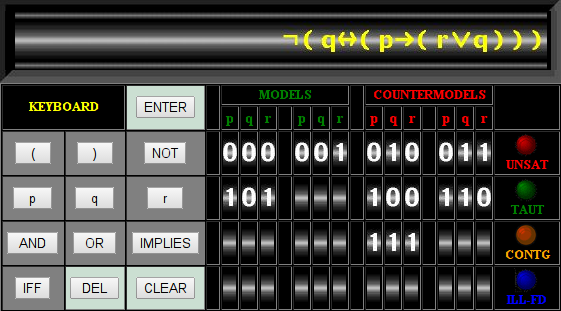
\includegraphics[width=\textwidth]{logiccalc.png}
    \caption{Propositional Logic Calculator}
    \label{logiccalc}
\end{figure}

\section{Previous Year Projects}

Once we have made more progress on our tool we will look into finding out what previous years did when they were assigned similar projects. We do not want to look into these this early in the project so we can generate our own implementation ideas as these projects will be very similar to ours.

\chapter{Parser}
\section{Parser Generation}

A parser generator is a tool which creates a parser from an inputted grammar. This is necessary so that we can parse the logic equivalences entered in to our application and create an internal tree representation.

\subsection{ANTLR4}

ANTLR is a widely used powerful parser generator that can be used to read, process, execute or translate structured text. It is used by a variety of companies such as Twitter for query parsing and Hadoop in data analysis systems. ANTLR supports a wide range of languages including Java making it a very suitable choice for our project.

From a grammar ANTLR generates a parser for that language and has the ability to automatically build parse trees representing the input. More interestingly, ANTLR also generates tree walkers which can be customised to visit the nodes of those trees and perform actions on those nodes. We use this functionality to build our own custom tree as described in Section \ref{sub:walker}.

ANTLR uses EBNF for its input grammar notation and uses an LL(*) parsing algorithm. This allows direct left recursion so that expressing our required syntax is easy and natural. 

\subsection{Alternatives to ANTLR4}
\label{sub:alternatives_to_antlr4}

ANTLR4 provides many benefits over previous versions and alternatives. ANTLR4 uses a new variation of the LL(*) parsing algorithm that was used in ANTLR3. It uses an adaptive algorithm that is much stronger than the static grammar analysis algorithm used in ANTLR3. This means that ANTLR4 will accept much more natural looking grammars and provides a lot more flexibility than in previous versions. The ability to write much more natural expression rules increases the usability as in previous versions it was often a struggle to write a grammar that ANTLR would accept. ANTLR4 aimed to focus more on ease-of-use and chose simplicity over complexity where possible. This is a large reason for choosing this parser generator over the alternatives.

Although there are a few other tools that can generate source code similar to ANTLR that you can load into a debugger and step through, none of them have adaptive LL(*) parsers as ANTLR4 does. Which means if we chose an alternative such as JavaCC we would need to configure our grammar to suit a weaker LL(k) parsing strategy. JavaCC is limited to the LL(k) class of grammars because it generates top-down parsers which means left recursion cannot be used. This would make generating the grammar more difficult and the result appear less natural.

Through our research we established that ANTLR4 provided the most sophisticated and easy-to-use parser generator for our project.

\section{Grammar}

\subsection{Propositional Logic}

The grammar we use with ANTLR can be seen in Listing \ref{expr.g4}. We only use propositional atoms between `a' and `r' because we don't need a whole alphabet of variables available and extending it to the whole alphabet would cause confusion with the logical or (`$\lor$') symbol. 

\begin{listing}[ht]
\begin{minted}[mathescape, frame=lines]{antlr}
grammar Expr;   

prog: expr;

expr: '(' expr ')'          #EXPR
    | '¬' expr              #NOT
    | expr BINOP expr       #BINOP_
    | expr '→' expr         #IMPLIES
    | expr '↔' expr         #IFF
    | ATOM                  #ATOM_
    |                       #ERROR
    ;

BINOP: ('∧' | '∨');
ATOM:  ('a'..'r' | '⊤' | '⊥');

\end{minted}
\caption{Expr.g4 grammar for Propositional Logic to be used by ANTLR}
\label{expr.g4}
\end{listing}

\subsection{Order of Precedence}

Precedence rules can be used as a way of reducing the number of necessary parentheses. We use these in our grammar to decide which connective is the main connective when parsing a non-atomic formula. The precedence of logical operators is defined in Table \ref{orderofprecendence}. The order of the grammar matches up with the order of precedence shown below, this is because ANTLR4 will choose the first rule that matches and this is how we maintain precedence.

\begin{table}[h]
\begin{center}
\begin{tabular}{|| c | c ||}
    \hline
    Operator & Precedence \\ \hline 
    $\lnot$  & 1 \\
    $\land$  & 2 \\
    $\lor$   & 3 \\
    $\to$    & 4 \\
    $\leftrightarrow$ & 5 \\ \hline
\end{tabular}
\caption{Order of Precedence for Propositional Logic}
\label{orderofprecendence}
\end{center}
\end{table}

\subsection{Parser, Lexer and Walker}
\label{sub:walker}

ANTLR automatically generates a parser and lexer for the grammar. The lexer tokenises the input source (the logical formula) into a token stream which can then be passed to the parser. A parse tree is generated by the parser which can be walked through by a custom walker. 

The custom walker extends the ANTLR generated listener to define methods for when the parser enters each rule defined in the grammar. For example, when the parser enters the {\tt NOT} rule, {\tt enterNOT()} is called. Equally, when that rule is exited, {\tt exitNOT()} is called. This allows us to walk through the parse tree and create our custom tree as we go.

An empty {\tt FormationTree} is passed through to the walker alongside the parse tree so the walker can build the tree up as the parse tree is walked through. Each time a grammar rule is entered the appropriate method in the walker is called to create that node in our tree. The structure of the tree is defined in more detail in Section \ref{sec:formation_tree}.

\subsection{Error Handling}
\label{sub:error_handling}

ANTLR provides an {\tt ANTLRErrorStrategy} interface for implementing a custom error handler to deal with syntax errors encountered during a parse by ANTLR-generated parsers. However, this has limited documentation and is a complex feature. Therefore, we have opted to relax the grammar by defining an error case so we can treat incorrect syntax as a semantic error instead.

As shown in Listing \ref{expr.g4} we define an {\tt ERROR} case which accepts any incorrect syntax. Once parsing is complete we walk over the tree using an {\tt ExprWalker} (described in Section \ref{sub:walker}) and when an error case is entered we can set an error flag in the tree. This enables us to manage the error later by displaying an error message to the user without the application throwing up errors.

\subsection{Extension to First Order Logic}

\chapter{Internal Tree Representation}

\section{Compiler}
\label{sec:compiler}

The compiler combines all of the generated and custom parts of the parser. We define a {\tt compile()} method to take the logic formula as input and parse it to create its tree representation. This is shown in Listing \ref{compile()}.

\begin{listing}[ht]
\begin{minted}{java}
public FormationTree compile(String expr) {
    CharStream input = new ANTLRInputStream(expr);
    ExprLexer lexer = new ExprLexer(input);
    CommonTokenStream tokens = new CommonTokenStream(lexer);
    ExprParser parser = new ExprParser(tokens);
    
    FormationTree tree = new FormationTree(null);
    ParseTree parseTree = parser.prog();
    
    ParseTreeWalker walker = new ParseTreeWalker();
    walker.walk(new ExprWalker(tree), parseTree);

    return tree;
}
\end{minted}
\caption{compile() function to convert a logical formula into a FormationTree}
\label{compile()}
\end{listing}

\section{Formation Tree}
\label{sec:formation_tree}

To build our internal representation of the logical formula we define a class {\tt FormationTree}. This is a slightly modified binary tree that stores the root node and an error flag as well as performing all of the tree operations required - such as adding a new node (detailed in Section \ref{sub:tree_operations}).

\subsection{Node Index}
\label{sub:node_index}

In the final application we will be manipulating individual nodes in the tree. If there are two nodes with the same values and subtrees we need to be sure we're applying a rule to the correct node. Therefore, it is essential that all nodes in the tree have a unique index.

TODO: Add diagrams with/without indexes to show why we require them and what could happen without.

\subsubsection{[Key, Depth] Pairs}

We represent this index as a [key, depth] pair. We define this pair using the three following principles:

\textbf{Principle 1:} A node's depth is defined as the level at which it is found in the tree. 

\textbf{Principle 2:} A node's key is defined by its horizontal position in its level with the leftmost node beginning at 0 and increasing incrementally.

\textbf{Principle 3:} Index's are also applied to gaps in the tree - where nodes could be placed in the future. So the leftmost leaf will only have a key of 0 if it is the child of all the leftmost nodes in the tree.

For example, a formula `a$\land$b' would only have three nodes - the `and' connective ($\land$) would have a key and depth of 0 and the atoms `a' and `b' would be at depth 1. As `a' is the leftmost node it will be assigned a key value of 0, and `b' will be assigned 1. The example's key and depths are shown in Figure \ref{keydepths}. 

By Principle 3 the incrementation of keys includes all gaps where it is possible for future nodes to be placed - so in our example it were possible for the node `a' to not exist, b would still have the index [1, 1] and would not be upgraded to [0, 1] as there is still a gap for a left child to exist in.

\begin{figure}[ht]
    \centering
    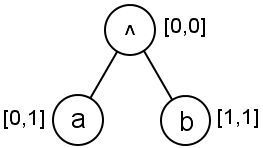
\includegraphics[width=0.4\textwidth]{keydepths.png}
    \caption{Tree representation of `a$\land$b' showing the key and depth at each node}
    \label{keydepths}
\end{figure}

\subsubsection{Binary Representation of Index}

The index of a node can be represented in binary to enable us to navigate around the tree easily. The depth represents how many bits should be read and the key defines the binary number. The depth is required so that two nodes with the same key cannot be read as the same. 

In the above example `$\land$' and `a' both have the same key, but their binary representations would be different. `$\land$' does not have a representation as it is the root (length of binary read is zero) and `a' would be 0. If `a' had a children the left child's index would be read as 00 and the right child's as 01. We go into more detail about navigating the tree using the binary representation of indexes in Section \ref{sub:tree_operations}.

\subsubsection{Determining Child and Parent Indexes}

Using this implementation of indexing not only guarantees that no two nodes will have the same index, but also we can easily work out the index of any child node, given we have the parent's index. For example, if we have a subtree of `c$\to$d' and we know the parent's ($\to$) index is [3, 2] and we want to calculate the index of the child node `c' we perform the following actions:

\begin{enumerate}
    \item \textbf{Key:} We perform a logical left-shift on the parent key (3 << 1 = 6)
    \item \textbf{Depth:} Increment the parent depth (2++ = 3)
\end{enumerate}

So the resulting index becomes [6, 3]. To calculate the right child `d' we can simply increment the key of the left child to become [7, 3].

We can also find the parent node's index given a child node by performing the opposite operations. A logical right-shift finds the parent key and decrementing the depth finds the parent depth.

TODO: Draw diagram of left-shift example

\subsection{Tree Operations}
\label{sub:tree_operations}

\subsubsection{Finding a Node}

Finding a node based on it's index is extremely straight forward using our node indexing scheme. We define a method {\tt findNode()} which simply steps through the tree using the binary representation of the index as a map.

For each level in the tree starting at the root node we take the left most bit of the key and this tells us whether we should take the left or right child route. An unset bit and a set bit represent the left and right children respectively. After we have taken that path and moved to the next level we use a mask to remove the left most bit from the key so that it does not conflict with the next level's left most bit.

Once the required depth is reached the current node is returned.

To find the node defined by index [1, 1] in Figure \ref{keydepths} we would begin at the root node and take the left most bit of the binary representation to determine our path. The binary representation of this node is 1. As the left most bit of this is 1 we take the right path putting us at the node `b'. This is at the required level so the tree walk completes and we return node `b'.

\subsubsection{Adding a New Node}

We define a method {\tt addNode()} to handle the addition of new nodes to the tree. The node passed in will already have its index set up so here we simply need to assign it to the correct position.

If the root of the tree does not exist then the node becomes the new root. Otherwise, we calculate the parent node's index as described in Section \ref{sub:node_index} and use {\tt findNode()} to obtain the parent node that will already exist in the tree. We set this as the new node's parent.

Either the parent node is a unary operator and we set the child of that node to be our new node, or it is a binary operator and we must determine if the the new node is a left or right child. If the node's key is divisible by 2 then the node is a left child, else it's a right child. We then set parent's child respectively. 

\section{Nodes}

Due to the nature of logical formulae we need to be able to differentiate between unary operators such as $\lnot$, binary operators such as $\to$ and atoms. We define a class {\tt Node} which all of these will extend to define the core functionality required from every node.

Every node in the tree must contain a key, a depth, a value and a parent (unless it's the root in which case the parent is null).

We define {\tt BinaryOperator}, {\tt UnaryOperator} and {\tt Atom} separately so we can set customised methods for each of them. Binary operators possess a left and right child, unary operators possess one child and atoms have none. The custom methods that require separate cases include a {\tt clone()} method to duplicate the node (used in applying certain rules - Section \ref{sec:the_rule_engine}), custom {\tt toString()} methods and methods for determining truth values (Section \ref{sec:generating_truth_tables}).

\chapter{Tree Manipulation}

The application requires a few key features concerning tree manipulation: the ability to apply logical equivalence rules to a tree, compare the equivalence of two trees and randomly generate trees.

\section{The Rule Engine}
\label{sec:the_rule_engine}

To handle the application of logical equivalences we define a series of rules that can be applied to individual nodes so long as they meet the required criteria for that rule. The {\tt RuleEngine} manages the application and selection of these rules employing a {\tt RuleApplicator} and {\tt RuleSelector} respectively.

TODO: Add screenshots of just the tree in app to show a walk through of how rules are applied.

TODO: Add Appendix with rules list

\subsection{Rule Selection}
\label{sub:rule_selection}

The {\tt RuleEngine} defines a method {\tt getApplicableRules()} to compute which rules are applicable to an individual node in a tree. This returns a {\tt BitSet} where each set bit represents a rule that can be applied.

Most of the rules can be put into categories (by operator) so only a subset of the rules need to be tested for a particular node. An example category is the `and' connective ($\land$) - if the selected node is an `and' connective then only the test for these rules should be performed as we know no other rules outside of that category will apply.

Within categories we define the tests for each rule individually. Some rules do not need any extra tests other than being assigned to a category. For instance the commutativity rule can be applied to any `and' or `or' operator node without any further tests being conducted. Whereas, the distributivity rule could be applied to an `and' operator only so long as one of its children was an `or' operator.

The {\tt RuleSelector} defines methods of testing for the properties required by the rules such as testing for idempotence which proceeds by checking that both subtrees of the node are equivalent. Each rule that can be applied to the current node has its index set in the returned {\tt BitSet}.

\subsection{Rule Application}
\label{sub:rule_application}

When the user selects an applicable rule the {\tt RuleApplicator} is used to apply that rule to the selected node. A function {\tt applyRuleFromBitSet()} is defined in the {\tt RuleEngine} to choose the correct manipulation to apply to the tree. It implements a large switch statement over the index of the rule to be applied with each case calling the necessary methods from the {\tt RuleApplicator}.

Some rules can require user input, for example in `$\bot \equiv$ a$\land\bot$' we require some input to decide which variable to use in the place of `a'. The selected variable can be passed in when applying the rule from {\tt BitSet}.

\section{Generating Equivalent Formulae}
\label{sec:generating_equivalent_formulae}

It is possible for a user to enter formulae manually, however, we also want to provide a quick option to automatically generate usable equivalent formulae.

\subsection{Random Formula Generation}
\label{sub:random_formula_generation}

When generating a logical formula we should be able to specify certain parameters such as how many variables and connectives are used. These parameters are used to generate different complexities of formulae for different difficulties.

The {\tt Compiler} is used to generate a random formula. The function {\tt generateRandomEquivalence()} takes the number of variables we want to use and the maximum depth of the tree to be generated. A selection of variables that can be used is then chosen (Section \ref{sub:variables}) and passed through to a function {\tt generateSubEquivalence()}. This recursively generates subformulae until the end criteria are fulfilled.

The end criteria are either the maximum depth or a random criterion has been reached. The random criterion adds an extra random factor so that we don't always get a balanced tree. This provides us with more interesting equivalences to work with. Currently the random criterion has a $\frac{1}{5}$ chance of succeeding because this produces nice looking results - trees which are generally not completely imbalanced but have a good level of variation to them. 

During each recursion if the end criteria has been met then we can randomly choose an operator and variables to assign to it and set this as a final subformula. Else, instead of assigning variables we call the function again and assign the returned results to the operator.

Random operators and variables are selected using instances of {\tt Random} from their respective lists. All the operators and a reduced selection of variables are available for use in the formula.

\subsection{Variables}
\label{sub:variables}

Initially all the variables would appear in a generated formula with the same probability. However, this proved to be a poor approach because you often ended up with many truth values ($\top$ and $\bot$) in the formula. This made the equivalences very easy to solve as you could usually just reduce both to their equivalent truth value. Proving the formulae were equivalent this way doesn't promote the users learning experience as they will repeatedly only use a very small subset of basic equivalences such as `a$\lor\top \equiv \top$'.

The solution to this problem was to assign probabilities to the variables. We define an enum {\tt Variable} (see Listing \ref{variableenum}) where all the entries have a value and a weight. The weight is defined on a scale of 0 to 100 with the higher weights being more likely to be chosen.

Initially all the atoms apart from the truth values are defined with a weight of 100 and the truth values are defined with a weight of 50 (so they will appear half as regularly as other variables). The application also provides the ability for a user to choose the probability they want these truth value atoms (`$\top$' and `$\bot$') to appear - to either increase or decrease the difficulty. When the user changes this probability the application will update the weights for the truth value variables.

The enum provides the method {\tt randomVariable()} to return a random variable based on their weights. A simple analogy for this method is to imagine a ruler where the maximum value is the sum of the weights and each weight is dashed on the ruler. If you randomly placed your finger somewhere along the ruler then the segment you land on becomes the variable you return. So variables with smaller weights are less likely to be selected.

\begin{listing}[ht]
\begin{minted}{java}
public enum Variable {
    A("a", 100), B("b", 100), C("c", 100), D("d", 100), 
        E("e", 100), F("f", 100), G("g", 100), H("h", 100), 
        I("i", 100), TRUTH("┬", 50), FALSE("⊥", 50);

    ...
}
\end{minted}
\caption{Variable enum defining values and weights for variables}
\label{variableenum}
\end{listing}

\subsection{Random Rule Application}

Applying random rules to a formula is used in generating an equivalent formula. When only one logical formula has been specified the user can request an automatically generated equivalence.

The second formula can be generated easily by repeated application of random rules. This guarantees that the generated formula will be equivalent to the first (because only applicable rules resulting in equivalence will be applied) and also allows us to set the difficulty of the proof based on how many steps there are between the two formulae.

There are two sections to the rule applications: choosing a random node and choosing a random rule. 

In our tree we define a method {\tt randomNode()} to randomly select a node. This method calculates the maximum depth of the tree by walking through the tree and returning the maximum depth found. A random level of the tree is chosen using an instance of {\tt Random} and the maximum depth before walking down the tree to that level - at each level the method arbitrarily picks a child to follow. When the selected random level is reached the current node is returned.

Once a node has been selected to perform a rule on we call {\tt getApplicableRules()} (see Section \ref{sub:rule_selection}) to obtain the {\tt BitSet} of applicable rules. From this the number of applicable rules is used with another instance of {\tt Random} to select a rule to apply. Some of the rules require user input, so we define a special case for these rules to randomly select a variable to be passed through to {\tt applyRuleFromBitSet()} (see Section \ref{sub:rule_application}) when applying the rule. If no user input is required then we pass through null.

\section{Truth Tables}
\label{sec:generating_truth_tables}

For a user to be able to complete a proof of their own custom equivalences we need to ensure that they are actually equivalent and the proof is completable before they begin. To do this we can use truth tables (defined in Section \ref{sec:truth_tables}).

\subsection{Generating Truth Tables}

{\tt TruthTable} contains a {\tt SortedSet} of variables, a {\tt LinkedHashSet<ArrayList<Integer>>} table (each {\tt ArrayList} represents a row in the table) and a {\tt String} formula. They can be represented as shown in Table \ref{table:generated_truth_table}. 

To generate the truth table we need to generate the values for the atoms (the first two columns of the example shown in Table \ref{table:generated_truth_table}) then apply them to the formula to find the final column's truth values.

\begin{table}[h]
  \begin{center}
    \begin{tabular}{ || c | c || c || }
      \hline
      a & b & a$\land$b \\ \hline
      0 & 0 & 0 \\
      0 & 1 & 0 \\
      1 & 0 & 0 \\
      1 & 1 & 1 \\
      \hline
    \end{tabular}
  \end{center}
  \caption{An example of a generated truth table}
  \label{table:generated_truth_table}
\end{table}

We use a {\tt SortedSet} to store the variables in so that when comparing two truth tables the columns will be in the same order to make comparisons easier. A {\tt LinkedHashSet} is required for the table because it has a predictable iteration order which is required for comparisons of tables. The same argument is used for using an {\tt ArrayList} for each row. This provides us with an ordered collection where we have precise control over where each element is inserted, enabling us to have easy access to the values in the rows - necessary for extending a table in certain cases.

\subsubsection{Creating Input Truth Values For Atoms}

For creating the first two columns of the table shown in Table \ref{table:generated_truth_table} we define a function {\tt createAtomicTruthValues()}. This takes the number of variables present in the formula (in this case 2 - `a' and `b') and calculates the number of rows that will be present in the table:

\begin{listing}[ht]
\begin{minted}{java} 
int rows = (int) Math.pow(2, numVars);
\end{minted}
\end{listing}

A new {\tt LinkedHashSet} table is created and for each row in the table and each variable we add a new entry as shown in Listing \ref{listing:create_truth_table}.

\begin{listing}[ht]
\begin{minted}{java} 
for (int i = 0; i < rows; ++i) {
    ArrayList<Integer> row = new ArrayList<Integer>();
    for (int j = numVars - 1; j >= 0; --j)
        row.add((i / (int) Math.pow(2, j)) % 2);
    table.add(row);
}
\end{minted}
\caption{Filling in table for atomic truth values}
\label{listing:create_truth_table}
\end{listing}

This produces the table shown in Table \ref{table:generated_atomic_truth_values}. A similar result is produced for any number of variables.

\begin{table}[h]
  \begin{center}
    \begin{tabular}{ || c | c || }
      \hline
      0 & 0 \\
      0 & 1 \\
      1 & 0 \\
      1 & 1 \\
      \hline
    \end{tabular}
  \end{center}
  \caption{The result of {\tt createAtomicTruthValues()}}
  \label{table:generated_atomic_truth_values}
\end{table}

\subsubsection{Determining Truth Value For The Tree}

TODO: Add diagram of tree example with truth values evaluated at each subequivalence

Each row of the table is used to evaluate the truth values of the formula for the final column in the table. We define the function {\tt createTruthTable()} to create the final truth table for the tree of a logical formula. This calculates the number of variables by walking through the tree and passes this value to {\tt createAtomicTruthValues()} to generate the atomic truth values required as described above. 

Looping through each row of the table allows us to compute the corresponding truth value for the formula. To compute the formula's truth value for that row a {\tt HashMap<String, Integer>} is created to map each variable to a truth value. The {\tt FormationTree} defines a method {\tt getTruthValue()} to calculate its truth value using this map.

The tree determines its truth value by recursively calling {\tt getTruthValue()} on its nodes beginning at the root. Using the example shown in Table \ref{table:generated_truth_table} for `a$\land$b': the root node is `$\land$' so the result would be a logical and of the left and right children. When {\tt getTruthValue()} is called on an atomic value it either returns 0 or 1 if its a `$\bot$' or `$\top$' respectively, else it returns the value defined for that atom in the map.

When evaluating the truth value for a formula the application uses shortcuts to reduce the amount of computation required. For example, when computing the truth value for the first row of our table [0, 0], where `a' and `b' both evaluate to 0 (or `$\bot$'), once the application knows the left child `a' is 0 there is no need to evaluate the right hand child because it's impossible for the overall truth value to be 1 (or `$\top$'). Therefore, the right hand evaluation is skipped.

The returned truth value is added to the end of its corresponding row in the table. Now the table looks as shown in Table \ref{table:final_generated_table} where the first two columns represents the truth values for the variables in our variables array and the final column represents the truth values for the whole formula.

\begin{table}[h]
  \begin{center}
    \begin{tabular}{ || c | c || c || }
      \hline
      0 & 0 & 0 \\
      0 & 1 & 0 \\
      1 & 0 & 0 \\
      1 & 1 & 1 \\
      \hline
    \end{tabular}
  \end{center}
  \caption{The result of {\tt createTruthTable()}}
  \label{table:final_generated_table}
\end{table}

The other operators use return their truth value using similar methods. The truth tables for all the used logical operators are defined in Table \ref{table:logical_operators}.

\begin{table}[h]
  \begin{center}
    \begin{tabular}{ || c | c || c | c | c | c | c || }
      \hline
      a & b & a$\land$b & a$\lor$b & a$\to$b & a$\leftrightarrow$b & $\lnot$a \\ \hline
      1 & 1 & 1 & 1 & 1 & 1 & 0 \\
      1 & 0 & 0 & 1 & 0 & 0 & 0 \\
      0 & 1 & 0 & 1 & 1 & 0 & 1 \\
      0 & 0 & 0 & 0 & 1 & 1 & 1 \\
      \hline
    \end{tabular}
  \end{center}
  \caption{Truth table for all binary and unary operators}
  \label{table:logical_operators}
\end{table}

\subsection{Testing Equivalence of Tables}
\label{sub:testing_equivalence_of_tables}

{\tt TruthTable} defines a method {\tt testEquivalence()} which compares its own truth table to another. There are four cases that could be possible when comparing truth tables:

\textbf{Case 1: } Both formulae have the same variables and are equivalent.

\textbf{Case 2: } Both formulae have different sets of variables and are equivalent.

\textbf{Case 3: } The formulae are not equivalent.

\subsubsection{Checking Tables Are Equal}

In the \textbf{Case 1} we could have two formulae such as `a$\land$b' and `b$\land$a'. These have contain identical sets of variables. They are equivalent if they contain the same set of variables and their truth tables are equal (Their truth tables are identical apart from the result formula).

Tables are checked for equivalence using {\tt tablesEqual()}. If the two tables to be compared aren't the same size the method immediately returns false to reduce computation time. If they're equal it loops through each row in both tables and checks that they're equal. If all the rows are contained in each table the method returns true.

\subsubsection{Different Variables and Differently Sized Tables}

The variable sets need to be compared in the previous case because the tables can be equivalent even if they use different variables. In this case the proof may or may not be solvable. For example, `a$\land$b' has an equivalent table to `p$\land$q' but we do not define any rules for replacing one atom in the tree with another so you would not be able to complete the proof. Whereas, `a$\land\lnot$a' and `b$\land\lnot$b' have equivalent tables and can be proven equivalent because they both reduce to `$\top$'.

However, a basic check to ensure the two variable sets are equal does not always work as there are cases where the variable sets will be different as described above. 

\textbf{Case 2} defines a case where both formulae are equivalent but have different variable sets. Another example of this would be `a$\land\top$' and `$\bot\lor$a' which both contain an atom not present in the other formula.

In this case we extend each table to include the missing variables (so both variable sets become equal) and then execute another comparison using {\tt testEquivalence()} where the tables will either fall into \textbf{Case 1} and be equivalent or \textbf{Case 3} and not be equivalent. 

Due to the rules such as the absorption rule it is possible for formulae with differently sized variable sets to be equivalent too. These equivalences can also be shown to have equivalent truth tables by table extension.

\subsubsection{Table Extension}

In this section we will be using `a$\land\lnot$a' and `b$\land\lnot$b' as our example formulae. The initial truth tables for each of these formula are shown in Table \ref{table:a_and_not_a}.

\begin{table}[h]
  \begin{center}
\begin{tabular}{ || c || c || }
      \hline
      a & a$\land\lnot$a \\ \hline
      0 & 1 \\
      1 & 1 \\
      \hline
\end{tabular}
\hspace{15mm}
\begin{tabular}{ || c || c || }
      \hline
      b & b$\land\lnot$b \\ \hline
      0 & 1 \\
      1 & 1 \\
      \hline
\end{tabular}
  \end{center}
  \caption{Truth tables for `a$\land\lnot$a' and `b$\land\lnot$b'}
  \label{table:a_and_not_a}
\end{table}

To be able to compare the truth tables of these formulae we need to extend them to include all the variables that appear in both formulae, the resulting tables should look as shown below in Table \ref{table:extended_a_and_not_a}.

%As you can see the variables and the tables are now equal and can be compared as in \textbf{Case 1}. This table extension is performed in {\tt testEquivalence} if the formulae fail the test for \textbf{Case 1}. 

First, a new variable set is created and the variables from both formulae are added to it as shown in Listing \ref{listing:create_new_variable_set}. In our example this set would become [a, b].

\begin{listing}[ht]
\begin{minted}{java} 
SortedSet<String> all = new TreeSet<String>();
all.addAll(variables);
all.addAll(v2);
\end{minted}
\caption{Creating the new variable set}
\label{listing:create_new_variable_set}
\end{listing}

Two new extended tables are created, the first initialised to the first original table and the second to the second original table. The function iterates through the new variable set and if a variable does not appear in one of the original sets it is added to its respective extended table using {\tt addVariable()} as shown in Listing \ref{listing:extending_tables}. 

Our example would need to extend both tables once until they had identical variable sets.

\begin{listing}[ht]
\begin{minted}{java} 
for (String var : all) {
    if (!variables.contains(var))
        extendedTable1 = extendedTable1.addVariable(var);
    if (!v2.contains(var))
        extendedTable2 = extendedTable2.addVariable(var);
}
\end{minted}
\caption{Extending the tables by adding new variables}
\label{listing:extending_tables}
\end{listing}

Adding a new variable to a table is done by duplicating each row and on each setting the value of the new variable to 0 and 1 respectively. The row [0, 1] in the formula `a$\land\lnot$a' would need a `b' variable added so would become two rows of [0, 0, 1] and [0, 1, 1] where the new variable has been inserted into the second column. The same would occur for the second row [1, 1].

Once both tables have been extended (Table \ref{table:extended_a_and_not_a}) the function calls {\tt tablesEqual()} on them to confirm that they have the same truth values and are equivalent.

\begin{table}[h]
  \begin{center}
\begin{tabular}{ || c | c || c || }
      \hline
      a & b & a$\land\lnot$a \\ \hline
      0 & 0 & 1 \\
      0 & 1 & 1 \\
      1 & 0 & 1 \\
      1 & 1 & 1 \\
      \hline
\end{tabular}
\hspace{15mm}
\begin{tabular}{ || c | c || c || }
      \hline
      a & b & b$\land\lnot$b \\ \hline
      0 & 0 & 1 \\
      0 & 1 & 1 \\
      1 & 0 & 1 \\
      1 & 1 & 1 \\
      \hline
\end{tabular}
  \end{center}
  \caption{Extended truth tables for `a$\land\lnot$a' and `b$\land\lnot$b'}
  \label{table:extended_a_and_not_a}
\end{table}

If this check also fails then the formulae are \textbf{Case 3} where they are not equivalent and the method returns false.

\chapter{Android VS Web Applications}

\section{Which Platform?}

In an ideal world it would have been very interesting and useful to have been able to build our application for multiple platforms - including for smartphones as well as tablets and the web. However, as we had a finite amount of time for this project it was initially obvious that focusing on one platform would provide us with a much more complete and robust final project.

The options were narrowed down by the fact we wanted to display the formation tree of the current formula as this would require a fairly large amount of screen space. Therefore, we opted not to build the application for a smartphone. If this were to be an extension we could simply remove the formation tree functionality to make the application usable on the smaller screen. This left us with the option of building for a tablet or a website.

Personal preference made the decision to choose an Android tablet as our tablet of choice because I had not had any experience programming with Android before and thought it would be a good skill to learn whereas I have programmed for iOS in the past. 

\subsection{Tablet Apps VS Web Apps}

\subsubsection{User Interaction}

The most obvious difference between an application on a tablet and on a computer is the difference in input methods. On a tablet a user uses gestures to interact with objects on the screen whereas on a computer a user can use the mouse to perform a variety of actions.

Obviously this is a key difference and would seriously affect the way the user would interact with the application. A tablet application would allow a more interactive application that would rely a lot more on user interaction such as using swiping gestures to move around the screen and selecting specific formula to undo back to that formula. This is because unlike on a computer a tablet does not have the ability to perform different types of clicks (left or right on the mouse) so the interaction would need to be well executed to be intuitive and easy-to-use. Therefore, choreographing the gestures and interaction on a tablet would be more difficult than on a webapp. 

\subsubsection{Portability}

A benefit of creating a tablet application is portability. As we are creating this application with the intention of it being a learning tool, the ability to use it easily and to be unintrusive and undisruptive in a lecture is a major bonus. A webapp could still be run on a laptop in this environment but they are generally considering to be more disruptive.

While a web application could be used on a tablet the user experience is much richer with native applications. The graphics and user interface used for web apps are not as smooth as one would find on a native app. This is because the graphics for a native app are already installed and therefore download speed during use does not need to be considered while developing\cite{androidwebappdifferences}.

Building a native app means that the application can utilize all the build in hardware on the phone and access internal data. This functionality is not available through a web app.

\subsubsection{Availability}

There are currently no Android applications that provide the functionality we have detailed so far. This is shown in Section \ref{chap:related_work} describing related work. Whereas there are more complex options available on a computer such as Pandora \ref{sec:pandora} even though they completely functionally the same as our application they are quite useful logic applications. 

\subsubsection{Learning Experience}

As I have not programmed any Android applications in the past I had a personal preference to creating an Android application. This would provide me with more to learn from the project unlike a web application which I have had a large amount of experience with.

\subsubsection{Decision}

In conclusion we decided to develop the application on an Android tablet device. Despite this being the more complex solution we believe that the application is more suitable to being used on a tablet and would be more likely to be used by students.

\chapter{Android}

Based on the Linux kernel Android is an operating system primarily designed for touchscreen mobile and tablet devices\cite{androidwiki}. The project responsible is the Android Open Source Project (AOSP) and is primarily lead by Google. The system provides a large user interface library and supports its graphics using the OpenGL-ES standard.

\section{Technical Background}

\subsection{Android Platform Components}

The Android system can be divided into four main levels, applications, the application framework, libraries and runtime, and the Linux Kernel (listed from top to bottom).

There are many default top level applications such as the Browser, Camera and Music. The application framework is an API allowing high-level interactions from applications to the Android system. Android libraries are used for many standard functions like web browsing and rendering graphics in the application framework and in the Dalvik runtime (Dalvik is the process virtual machine in Android). The Linux kernel acts as a communication layer for the underlying hardware.

When developing for Android a developer will only tend to work on the top two layers.

\subsection{Applications}

Applications extend the functionality of Android devices and are primarily developed in Java using the Android SDK. The SDK provides an extensive set of development tools and there is plenty of documentation available.

Users of an Android device can download third party applications through an app store such as Google Play. There is a growing number of third party applications and the app stores allow a user to browse, download and update any applications published suitable for their device.

There were more than one million applications available for download from the Google Play Store as of July 2013\cite{appstoredownloads}. 

\subsection{Memory Management}

As with most mobile and tablet devices most Android devices are battery powered. Unlike desktop operating systems such as Windows, Android is designed to keep power consumption low. This is because desktop operating systems can make the assumption that they will be connected to unlimited mains electricity. 

To keep power consumption at a minimum Android will set apps to idle when they are no longer in use, suspending them so they don't consume battery or processing power. Keeping apps idle means that they do not need to be closed and reopened when a user wants to access them again which also helps reduce power consumption.

\subsection{Market Share}

Android's main competitor in the mobile platform market is Apple's iOS. In research conducted in the fourth quarter of 2012, Kantar Worldpanel Comtech showed sales of all Android smartphones worldwide outpacing the iPhone by a huge margin: 70 percent to 21 percent of the smartphone market\cite{androidstats}.

In the tablet market the iPad dominated Android's $7\verb+"+$ tablets with 53.8 percent to 42.7, which is lower than Android's smartphone market but steadily increasing.

\section{Features}

\subsection{Graphics and Widget Library}
\label{sub:graphics_and_widgets}

Android does not use the Swing library or the Abstract Window Toolkit (AWT) used in most Java applications. Instead the graphical user interface for an Android app is built using a hierarchy of {\tt View} and {\tt ViewGroup} objects. The framework employed is similar to Swing but based around {\tt View} objects rather than {\tt JComponent} objects.

{\tt ViewGroup} objects are hidden containers used to define how the child views are positioned. Buttons and text fields are some examples of {\tt View} objects, they are UI widgets that manage what a user can see and do on the screen. {\tt View} and {\tt ViewGroup} components can either be defined in XML or programmatically.

Widgets require the Android application's {\tt Context} to be provided at creation. The {\tt Context} of an application provides global information about its environment. As the name suggests, its provides the context of the current state of the application allowing newly created objects to understand what has occurred. It can be used to obtain information about another part of the program such as another {\tt Activity}.

\subsection{Activities}
\label{sub:activities}

An {\tt Activity} is the base for the user interface in Android, it represents the presentation layer which a user will see. Android applications tend to have multiple activities which are switched between during runtime.

Often activities will be presented as a full-screen window but they can also be used as floating windows or embedded inside other activities (implementing {\tt ActivityGroup}). All {\tt Activity} classes must be declared in the Android manifest file. This is an XML file that holds all the essential information the application requires before it can run any code.

When a new activity begins it is pushed onto the `back stack' and the previous activity is stopped. As the stack has the standard `last in, first out' structure when a user presses the back button the current activity will be popped off and the previous activity is resumed. 

\subsection{Fragments}
\label{sub:fragments}

A {\tt Fragment} is a piece of an application's UI that can be placed inside an activity. Each fragment defines its own lifecycle (with its own methods: {\tt onCreate()}, {\tt onPause()}, etc.). Although the lifecycle is reliant on its activity (if the activity is stopped then no fragments inside the activity may be started) a fragment is able to respond independently to events.

Fragments allow for modularisation of the layout code so that the user interface is more easily adjustable.

\subsection{Intents}
\label{sub:intents}

Intents are used as a link between two activities for transferring data between them. Each {\tt Intent} is an asynchronous message suppling an action and data to the new activity. They are most often used for starting another activity and providing that activity with whatever information it requires from the previous. Intents are extremely useful as they allow the creation of a loose binding between two separate components.

\subsection{Layouts}
\label{sub:layouts}

The layout is a view group which defines the visual structure in an activity or widget. A layout can be declared in an XML activity or fragment file or the layout elements can be instantiated at runtime. We can view a visual representation of the layout of an XML file in the graphical layout editor in Eclipse thanks to the ADT plugin. Declaring the layout in the XML file allows for better seperation of the presentation and behaviour of the app. Different XML layouts can be defined for different screen sizes or screen orientations. 

There are a few different types of layout that can be used including {\tt LinearLayout} and {\tt RelativeLayout}. {\tt LinearLayout} aligns all of its children either vertically or horizontally and {\tt RelativeLayout} displays its child views in their relative positions. There are other types of layout that will be described as they are used in the application.

Every layout requires layout parameters, these control how the layout will appear on the screen. As layouts are view groups they can be nested inside each other. Defining layout parameters allow us to control how much of the screen each of these layouts take up.

\subsection{Multi-Touch Gestures}
\label{sub:gestures}

The user interface is based around direct manipulation. This means using touch inputs that are intended to correspond to real-world actions, for example swiping, pinching and tapping to control on-screen events. The response to user actions is designed to be immediate and provides a fluid touch interface. It often provides haptic feedback (forces, vibrations or motions) to the user using the vibration capabilities.

Android takes advantage of internal hardware such as accelerometers, gyroscopes and proximity sensors in some applications to respond to other user actions, such as re-orientating the screen from portrait to landscape.

\section{Difficulties Developing For Android}

During development of the application we encountered some difficulties specific to Android which we would not have experienced if we had developed a web application. There are detailed below and will be referencing aspects of the project detailed later in the report.

\subsection{Screen size and Scrolling}

Tablets have a limited screen size compared to a computer screen. Although we have established that the screen size would be suitable for displaying the formation trees of the equivalences it does present the difficulty of moving around the application. Android provides a scrollable view that allows the view to scroll either horizontally or vertically, but not both. Nested scrollable views are not allowed as the application would not be able to understand which view you were trying to scroll through.

This is problematic as it is possible for a large formation tree to be larger than the width of the screen. We could not set the scrollable view to scroll horizontally because we require vertical scrolling for long equivalence proofs. On a computer this would be an easy solution as nested scroll boxes are easy to implement.

TODO: Add the solution

\subsection{External Libraries}

Using external libraries with Android proved to be much more of a challenge than expected. This was especially evident when looking for an external library used for drawing attractive trees. Most of the libraries available hooked straight into Java's Swing components and so huge amounts of the library would need to be rewritten for it to function on Android.

This meant that any external libraries used needed to separate the core functionality from the actual rendering to be usable. Even then needed some tweaking was required to get them to function correctly. An example of this challenge is described in our formation tree representation in Section \ref{sub:abego_treelayout}.

\subsection{Custom Features}
\label{sub:custom_features}

Android provides the ability to generate your own custom features when the ones you want are not available. Such as the custom keyboard described in Section \ref{sec:custom_keyboard}. These features would not need to be implemented on a web app as the computer would already provide all of them. Implementing the custom keyboard was a difficult process as the {\tt KeyboardView} we needed to extend is not well known. Although there is documentation on the {\tt KeyboardView} there are not many examples and there are some issues in when to show the keyboard.

Designing our own {\tt KeyboardView} has the downside that it is a {\tt View} and as such is a part of the layout in an Activity. This means the {\tt View} will obstruct all the layouts implementing it but we are in complete control of our application, keyboard included.

For unknown reasons {\tt KeyboardView} is not part of any automatically found package (returning a {\tt java.lang.NoClassDefFoundError}) meaning the full path to the class is required. Therefore, the graphical layout editor (which shows a graphical representation of the XML file) cannot show a representation of the keyboard making the design process slightly more difficult.

One of the most complex issues was making the keyboard appear at the right time, and even more difficult was making the standard keyboard invisible at the same time. Android is very persistant in having the standard keyboard appear. The workaround was to set the input type of the text box as {\tt TYPE\_NULL} (telling Android we wouldn't be editting that text box), however this hides the cursor meaning we needed to add our own cursor keys to our keyboard. This is currently considered a bug.

\subsection{Less Experience}

Developing for Android proved to be a steep learning curve as I had never developed for it before. This definitely proved to be a hurdle in the progress of the application and development proceeded a lot more slowly compared to if we had developed a web application.

\chapter{The App}

\section{Activities}

As defined in Section \ref{sub:activities}, activities can be used to represent each screen in the application. In this application there are three activities: {\tt MainActivity}, {\tt EnterEquivalenceActivity} and {\tt BeginEquivalenceActivity}.

\subsection{Main Activity}

{\tt MainActivity} controls the first screen the user sees when they start up the app. This allows the user to change the settings and choose either propositional or first order logic, shown in Figure ...

TODO: take screen shots of app

The fragment (see Section \ref{sub:fragments}) XML file {\tt fragment\_main} contains the widgets you can see in Figure ... These are defined as {\tt TextView}, {\tt Button}, {\tt SeekBar} and {\tt Spinner} widgets. {\tt TextView} and {\tt Button} widgets are self-evident, the {\tt Spinner} is used to create the dropdown menu to select the difficulty and the {\tt SeekBar} is used for the slider that controls the probability of truth atoms appearing in the generated formula.

When the `Propositional Logic' button is clicked {\tt startPropositional()} is called. This creates an {\tt Intent} (see Section \ref{sub:intents}) to start a new {\tt EnterEquivalenceActivity}. The difficulty (Section \ref{sec:difficulty}) and selected probability (Section \ref{sub:variables}) of truth values are added to the intent and it starts the new activity.

TODO: when `First Order Logic' is clicked

\subsection{Enter Equivalences Activity}

{\tt EnterEquivalencesActivity} allows the user to either manually enter or randomly generate the formulae to prove equivalent. As shown in Figure ... the XML fragment {\tt fragment\_enter\_equivalences} defines two {\tt EditText} widgets to manually enter the formulae. These widgets use a custom keyboard for entering logical symbols and variables (Section \ref{sec:custom_keyboard}). Two `Randomise' buttons are defined to automatically generate equivalences (Section \ref{sec:app_generation_of_equivalences}).

Upon the `Start' button being pressed the activity will check the two formulae are equivalent (Section \ref{sub:equal_equivalences}). If there is a problem with the formulae entered (either they are not equivalent or they have a syntax error) then the appropriate error message will be shown (Section \ref{sub:error_messages}). If the formulae are equivalent a new {\tt Intent} will be created to begin a new {\tt BeginEquivalenceActivity}. The intent will carry the two formulae to the new activity so that the user can begin the proof.

TODO: more screenshots!

\subsection{Begin Equivalence Activity}

The XML file {\tt fragment\_being\_equivalence} employs a {\tt ScrollView} as its outer layout, this is a specific type of view group extending {\tt FrameLayout}. A {\tt FrameLayout} surrounds one child (usually another layout) containing its entire contents, {\tt ScrollView} then allows us to scroll through the content so the layout can be bigger than the physical display. 

A {\tt LinearLayout} (Section \ref{sub:layouts}) is used as the child of the {\tt ScrollView} which then contains all the widgets required for completing the proof. This layout consists of two main sections, one for each formula. The start formula is placed at the top of the layout working down and the end formula is placed at the bottom working up. Each end displays its current formation tree (Section \ref{sec:formation_tree_representation}) and allows the user to undo or redo rules (Section \ref{sec:undo_redo}). This display is shown in Figure ...

TODO: An example of completing a proof shown somewhere.

TODO: last screenshot
 
\section{Difficulty}
\label{sec:difficulty}

The selected difficulty only affects the proof when formulae are randomly generated because when a user manually enters their own formulae they are in complete control over what they want to prove.

\subsection{Difficulties}

The user can choose a difficulty from either beginner, intermediate or hard in the settings of the application. Each of the difficulties have set values for their parameters which are used in generating formulae. 

\subsection{Parameters}

The parameters used in generating equivalent formulae are the number of variables that can appear in the inital formula ({\tt numVars}), the maximum depth of the formula's tree ({\tt depth}) and the number of rules we will apply to the initial formula to generate two formulae equivalent to the original ({\tt numRules}).

\vspace{5mm}
\begin{center}
  \begin{tabular}{ | c | c | c | c | }
    \hline
    Difficulty & numVars & depth & numRules \\ \hline
    Beginner & 3 & 0 & 3 \\
    Intermediate & 5 & 1 & 4 \\
    Hard & 10 & 2 & 5 \\
    \hline
  \end{tabular}
\end{center}
\vspace{5mm}

TODO: In this table a depth of 0 actually means a ??? - Explain!

TODO: See \ref{sec:app_generation_of_equivalences} for screenshots of generated equivalences from difference difficulties

\subsection{Probability of Truth Values}

Initially the probability of the truth values was tied to the difficulty the user selected, however it was suggested that it could be beneficial to the user to have direct control over this parameter. 

As described in Section \ref{sub:variables} the user has the ability to set the likelihood of the truth values being chosen (up to the same amount as other variables). The user can set this value using the {\tt SeekBar} in {\tt MainActivity}. The {\tt SeekBar} has a maximum value of 100 (so at maximum it will be equally likely to be chosen as other variables) and a default value of 50 (half as likely). This value is passed through with the other parameters when generating new formulae.

\section{Random Generation of Equivalences}
\label{sec:app_generation_of_equivalences}

{\tt EnterEquivalencesActivity} has a compiler (Section \ref{sec:compiler}) and a rule engine (Section \ref{sec:the_rule_engine}) which is used to generate formulae and apply rules.

TODO: Add screenshot of EnterEquivalencesActivity or reference previous screenshot

The top and bottom `Randomise' buttons call {\tt randomiseStart()} and {\tt randomiseEnd()} respectively. These functions simply call the {\tt randomise()} function and pass through which text box it is trying to generate a random formula for.

There are three possible cases when one of these buttons have been clicked:

\textbf{Case 1:} Neither text box contain formulae and one needs to be generated from scratch.

\textbf{Case 2:} The other text box contains a valid formula and an equivalent one needs to be generated.

\textbf{Case 3:} The other text box contains an invalid formula and an error will be thrown.

The {\tt randomise()} function takes both text boxes as parameters, the first being the text box we want to display the generated formula in and the second the other text box. It then determines if the other text box is empty and acts accordingly.

\subsection{The Initial Formula}

The {\tt Compiler} is used to generate a random formula when a `Randomise' button is clicked (Section \ref{sub:random_formula_generation}) using the user specified parameters.

Previously, this generated formula would be set as the new formula in the text box corresponding to the button clicked. This gave an unfortunate side effect when a second equivalence was generated (\textbf{Case 2}), where it would usually be longer than the first - due to the fact that there are more rules which increase the size of a formula. 

This is not a problem if the user begins the proof immediately, but if the user clicks the first randomise button again the app would generate a formula equivalent to the previously generated longer formula creating a longer again formula. Repeating this by alternating clicks on each button resulted in the formulas continuously increasing in length disregarding the difficulty set.

The solution to this was to set the generated formula as an \textit{initial formula} to which rules would be applied to generate any required formulae.

\subsection{Generating Equivalent Formulae}

In \textbf{Case 1} the other text box has nothing in it so a new formula needs to be generated by the compiler. If there is already something in the current text box it will be overwritten. The initial formula is remembered by the activity, compiled into a tree and a number of random rules are applied to the tree (depending on the difficulty). This new tree's formula is set as the first formula in the text box.

In \textbf{Case 2} there are two sub cases. Either the other formula was generated by the activity and an initial formula has been set, or it was manually inputted and there is no initial formula. If no initial formula is set then it is set to the manually inputted formula in the other text box.

The initial formula is then compiled into a tree and has random rules applied to it (as above in \textbf{Case 1}). This newly generated tree has its formula set to the textbox.

TODO: Screenshots of generated formulae

\textbf{Case 3} occurs when the initial formula has been set from a manually inputted formula with incorrect syntax. In this case the parsing of the formula will fail and an error flag will be set. When this flag is set an error message will be shown informing the user of their error and no equivalent formula will be generated.

TODO: Screenshot of error message

\section{Custom Keyboard}
\label{sec:custom_keyboard}

In the application we enter formulae in alpha numeric fields. Android provides context sensitive soft keyboards for entering text so different keyboard appear in different situations. However, it does not provide a keyboard for logic symbols meaning a different keyboard is required.

Other than the standard keyboards provided by Android there are manufacturer keyboards and user installed keyboards. The manufacturer keyboards are a more simple reduced version of the Android keyboards also without logic symbols. User installed keyboards allow a developer to have complete control over the keyboard but end users of the application would have to also install the keyboard service. Installing a keyboard service would be an inconvenience for the user and also presents a security risk because everything that passes through the keyboard can be tracked by the application including passwords. 

\subsection{Keyboard View}

Android has a {\tt KeyboardView} (difficulties with using this described in Section \ref{sub:custom_features}), this is a view that allows us to define the keys the keyboard displays. The keyboard is made up of rows of keys. Each key is associated with a label and a code. The label defines what is shown on the key button and the code is passed to the app when the key is pressed. 

The keys are defined in {\tt logickbd.xml} and when a key is pressed the key's code is passed to the {\tt CustomKeyboard} class. A key listener is used in {\tt CustomKeyboard} to detect when a key is pressed, finds the view in focus and ensures it's an {\tt EditText} (else it aborts) then executes an action based on the key's code.

TODO: Keyboard screenshot  

\subsection{Keys}

If a variable or symbol key is pressed then the corresponding symbol is inserted into the text box. Undo deletes the last value and clear deletes everything in the text box. Hide is used to hide the keyboard and the arrow keys are used to move the cursor left and right.

TODO: Why we need cursor keys 

\subsection{Hiding The Keyboard}
\label{sub:hiding_the_keyboard}

TODO: Reference difficulties/don't repeat yourself

\subsection{Registering Text Boxes}

Each text box that requires the logic keyboard needs to be set up to use it. The function {\tt registerEditText()} enables the application to register multiple text boxes to use the keyboard.

First this function sets the text box's listeners to show the custom keyboard when the text box is selected and has focus. It also hides the standard keyboard, sets up the new cursor and turns spell check off.

\section{Truth Tables}
\label{sec:app_truth_tables}

After two formulae are entered (either manually or generated) the user can click the `Start' button. This button is linked to {\tt startEquivalence()} which uses truth tables to check the formulae are equivalent and creates an intent to start a new activity.

\subsection{Equal Formulae}
\label{sub:equal_equivalences}

The function {\tt startEquivalence()} finds the {\tt EditText} boxes holding the formulae by their ids defined in the XML file and retrieves the text within them. These two formulae are both compiled into their {\tt FormationTree} and a truth table (Section \ref{sec:truth_tables}) is generated for each tree. 

If these truth tables are equivalent then a new intent is created to carry the equivalences to the new {\tt BeginEquivalenceActivity}. Before the formulae are added to the intent we set the equivalences to the {\tt String} representation of their respective trees. This is to deal with the case where no brackets have been used and have been implied by the parser. Setting the formulae to the {\tt String} representation of the tree adds in the brackets where they have been implied to avoid confusion later on. The two equivalences can then be added to the intent and the new activity is started.

TODO: Add screenshot example of no brackets in formulae

\subsection{Error Messages}
\label{sub:error_messages}

An error message is displayed to the user in certain cases. A function {\tt setErrorMessage()} is defined to set the error message to the passed in text and make the message visible.


\subsubsection{No formulae have been entered}

If the start button is clicked and both formulae have nothing in them then an error message saying \textit{`Please enter two equivalent formulae'} is set.

TODO: Add screenshot of error message

\subsubsection{Incorrect Syntax}

Section \ref{sub:error_handling} describes how the parser handles syntax errors. When incorrect syntax is found it allows the incorrect formula to be parsed and sets a flag in the resulting tree. Before creating truth tables for each tree if either has its error flag set then the error message \textit{`Incorrect syntax'} is set.

TODO: Considered highlighting which symbol is incorrect?

\subsubsection{Formulae are not equivalent}

If the test for equivalent truth tables fails then the intent is not created and the error message \textit{`Not equivalent'} is set.

\section{Formation Tree Representation}
\label{sec:formation_tree_representation}

\subsection{The Formation Tree}

Each logical connective in an formula can be written enclosed in parentheses. For example:

\begin{center}
(a$\to$b)$\land$$\neg$a \ can be written as \ ((a$\to$b)$\land$($\neg$a))
\end{center}

Due to this property we can create a binary tree unique to each proposition; this is called a formation tree. Each connective and propositional atom is represented by a node and a leaf respectively. This provides a clear and attractive way of displaying the formula but is too expensive for every day use. In our application we wish to display the formation tree of the current equivalences.

Displaying the formation trees allows a user to see an interactive representation of the equivalences where touching the nodes and leaves in the tree allows the user to apply rules to various parts of the tree.

\subsection{The NP-Complete Problem}

When planning to draw the formation trees to the app we assumed there would be a simple, classic algorithm for drawing neat, aesthetically pleasing trees. However, we discovered the problem was not that simple. Drawing an attractive Tree layout is an NP-complete problem\cite{npcompletetrees} and there are many tree-drawing algorithms attempting to solve the problem of drawing attractive trees. We reviewed many of these algorithms to find one suitable to use.

\subsection{What Makes An Attractive Tree?}

Although generating an attractive tree is a matter of taste, certain principles are widely agreed upon to be key to drawing an aesthetically pleasing tree. The first three are taken from Wetherell and Shannon's tree drawing algorithm for producing tidy drawings using the smallest width possible\cite{tidierdrawingsws}.

\textbf{Aesthetic 1}: Nodes at the same level of the tree should lie along a straight line, and the straight lines defining the levels should be parallel. 

\textbf{Aesthetic 2}: A left son should be positioned to the left of its father and a right son to the right.

\textbf{Aesthetic 3}: A father should be centered over its sons.

Although not mentioned in the original article, Aesthetic 1 was also meant to guarantee the edges in the tree do not intersect except at the nodes by requiring that the relative order of nodes over any level be the same as the level order traversal of the tree. Wetherall and Shannon's algorithm is fairly basic and has a deficiency that compromises the overall attractiveness of the resulting tree. It produces drawings that could be made narrower within the constraints of the aesthetics and are not entirely pleasing to the eye - nodes in certain subtrees are drawn too far apart due to the fact that their shape is influenced by the positioning of nodes outside that subtree. This leads to the asymmetry of the resulting tree. Therefore when Reingold and Tilford\cite{tidierdrawingsrt} set out to create a better tree drawing algorithm they introduced a fourth aesthetic:

\textbf{Aesthetic 4}: A tree and its mirror image should produce drawings that are reflections of one another; moreover, a subtree should be drawn the same way regardless of where it occurs in the tree.

Fulfilling this aesthetic requires us breaking Wetherell and Shannon's aim of minimum width so that all all isomorphic subtrees are drawn the same. This is considered a more important principle than using the minimum width as our main aim is to create an attractive tree. This is an acceptable drawback as Supowit and Reingold proved that determining the minimum width under these aesthetics is NP-hard\cite{complexityofdrawingtreesnicely}. Therefore, we can use Reingold and Tilford's algorithm to draw our formation tree to produce an attractive result. 

\subsection{Reingold and Tilford's Algorithm}

The proposed algorithm was based on the following heuristic: 

``Two subtrees of a node should be formed independently, and then places as close together as possble''\cite{tidierdrawingsws}.

This is applied during a postorder traversal of the tree by taking the two subtrees of a node and calculating the contours of those subtrees. The two subtrees are then positioned so they overlap at their roots before moving them apart until no two points are touching. This is done recursively at each level moving down the levels of the tree until the bottom of the shortest subtree is reached. Once the process is finished the position of the subtrees can be fixed relative to their parent node which is centered over them. Once the postorder traversal is complete a preorder traversal occurs to convert the relative positions to absolute coordinates.

\subsection{Walker's Algorithm}

Extending Reingold and Tilford's algorithm to to rooted ordered trees of unbounded degree as described in their paper produces layouts where some subtrees of the tree could have been dispersed better to create a more attractive layout. In 1990 Walker's algorithm solved this problem by spacing out subtrees whenever possible, however in the initial algorithm presented the runtime was quadratic. Walker's algorithm was improved upon by Christoph Buchheim, Michael J\"unger and Sebastian Leipert so it would run in linear time\cite{improvingwalkers}. This is the algorithm we use in our application. 

\subsection{Abego TreeLayout}
\label{sub:abego_treelayout}

TODO: Add challenge of using it on Android

Abego TreeLayout is an external library which efficiently creates compact and highly cusomisable tree layouts. It is based on Walker's algorithm with the enhancements previously mentioned suggested by Buchheim, J\"unger, and Leipert\cite{treelayoutlineartime}. The software builds tree layouts in linear time so that even trees with many nodes are built quickly. TreeLayout separates the layout of the tree from the actual rendering, therefore it is suitable for drawing trees in an Android application because it is not limited to a specific output or format.

\begin{figure}[ht]
    \centering
    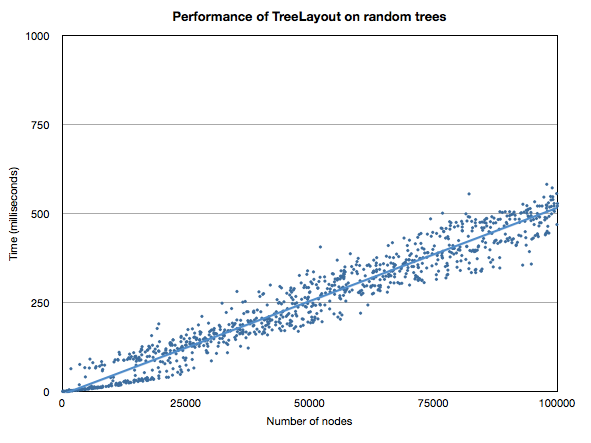
\includegraphics[width=\textwidth]{abegolineartime.png}
    \caption{Illustrates the linear time behaviour of the Abego TreeLayout algorithm\cite{abegolineartime} and shows the applicability for large numbers of nodes. (Graph taken from the Abego TreeLayout documentation).}
    \label{abegolineartime}
\end{figure}

\subsection{Drawing the Formation Tree}

We created a custom view DrawView to draw the trees to the screen in the application. This is created by simply extending the Android View class and overriding the {\tt onDraw()} function. To add a custom view to our user interface we also need to define custom attributes in a resource element as shown in Listing \ref{drawviewxml}.

\begin{listing}[ht]
\begin{minted}{xml}
<declare-styleable name='DrawView'>
    <attr name='showTree' format='boolean' />
</declare-styleable>
\end{minted}
\caption{DrawView resource element}
\label{drawviewxml}
\end{listing}

In {\tt onDraw()} we determine whether we are drawing the top or bottom formation tree and call {\tt setUpTreeLayout()} (shown in Listing \ref{setuptreelayout}) which uses the Abego TreeLayout to manage the layout.

To use TreeLayout we create a {\tt TreeLayout} instance with our tree (accessible through the {\tt TreeForTreeLayout} inferface), a {\tt FixedNodeExtentProvider} (defines a fixed size for each node) and a {\tt DefaultConfiguration} (configures the layout by defining parameters such as {\tt gapBetweenNodes} and {\tt gapBetweenLevels}).

\begin{listing}[ht]
\begin{minted}{java}
public void setUpTreeLayout(Location location) {
    DefaultConfiguration<Node> configuration = new 
            DefaultConfiguration<Node>(gapBetweenLevels, 
            gapBetweenNodes, location);

    FixedNodeExtentProvider<Node> nodeExtentProvider = new 
            FixedNodeExtentProvider<>(20, 20);
    treeLayout = new TreeLayout<Node>(tree,
            nodeExtentProvider, configuration);

    ...
}
\end{minted}
\caption{setUpTreeLayout() is called by onDraw() in DrawView}
\label{setuptreelayout}
\end{listing}

TreeLayout calculates the position of each node so we can then paint the nodes and edges to the screen using Android Canvas.

\subsection{Responding to Touch Events}

By overriding {\tt onTouchEvent()} in DrawView we can get the event action performed on the view. Using this we can check if the touched position is within the bounds of any of the nodes drawn to the screen. If the position is within the bounds of a node we display applicable rules for that node by calling {\tt setRules()} on the current activity ({\tt BeginEquivalenceActivity}). Selecting a node also forces a redraw so that we can highlight the selected node.

\section{Rule Application}

\subsection{Rule Display}

The rules are displayed in a PopupMenu on screen either above or below the selected tree. The rules are generated by the {\tt RuleEngine} as described in Section \ref{sec:the_rule_engine}.

Calling {\tt setRules()} adds the generated rules iteratively to the PopupMenu. If the rule requires user input (eg. $\top := \bot \to a$) a SubMenu is created with the variables that can be applied as shown in Listing \ref{rulessetup}. Each entry in the PopupMenu contains the String representing the rule and the rule key. The key is required so we know which rule to apply on touch events.

\begin{listing}[ht]
\begin{minted}{java}
public void setRules(SparseArray<String> rules, Node 
        selected, FormationTree selectedTree) {
    ...

    int key;
    for (int i = 0; i < rules.size(); ++i) {
        key = rules.keyAt(i);

        if (key < min_user_input_required) {
            rulesList.getMenu().add(Menu.NONE, key, 
                    Menu.NONE, rules.get(key));
        } else {
            SubMenu sub = rulesList.getMenu().addSubMenu(
                    Menu.NONE, key, Menu.NONE, rules.get(key));
            SortedSet<String> vars = topTree.getVariables();
            vars.addAll(bottomTree.getVariables());

            for (String v : vars) {
                sub.add(Menu.NONE, key, Menu.NONE, 
                        rules.get(key) + " using " + v);
            }
        }
    }
    rulesList.show();
}
\end{minted}
\caption{Rules being added to the rulesList PopupMenu in setRules}
\label{rulessetup}
\end{listing}

\subsection{Responding to PopupMenu Touch Events}
\label{sub:responding_to_popupmenu_touch_events}

Overriding {\tt onMenuItemClick()} in {\tt BeginEquivalenceActivity} allows us to determine which item was selected from the PopupMenu and and apply that rule to the selected node. We can determine which rule should be applied by taking the key of selected item and applying that rule from our {\tt BitSet} of rules using the {\tt RuleEngine} (Section \ref{sec:the_rule_engine}).

Applying a rule to the selected node adds a new {\tt TextView} to the respective list of equivalences (either top or bottom). Once the rule has been applied the application will check for completion and cycles (Section \ref{sub:detecting_cycles}). If either are found a {\tt Toast} (a simple popup for displaying feedback) will be displayed alerting the user.

We also override {\tt onDimiss()} so that when a user dismisses the PopupMenu without selecting a rule we can also redraw the formation tree to deselect the selected node.

\section{Undo/Redo}
\label{sec:undo_redo}

A main feature of the application is intuitive undo and redo functionality. Selecting a previous equivalence in the list (from either end) should display the formation tree for that equivalence and grey out the undone equivalences below as shown in Figure ...

TODO: Screen shots

\subsection{Adding A New Formula}

When a new formula is added it is either added to the top or bottom layout depending on where the call has come from. Throughout this section we will refer to the top layout, however the bottom layout functions in a similar way with layout inverted.

To add the new formula the top layout {\tt addTextViewToTop()} is called. This sets up the text view by setting its layout parameters and customises how the view will look on screen. Its id is set to the number of equivalences in the layout so far - which is used for ordering the equivalences when they are undone and redone.

Each text view has an {\tt OnClickListener} set, the function of this will depend on where the text view is in the layout. If the text view displays the current formula then clicking it will simply hide/show the current formation tree. If the text view is a previous equivalence before the current formula then on click the application will undo up till this equivalence. If the text view is below the current formula then it's been previously undone and clicking it again will redo up to and including this equivalence.

After the {\tt OnClickListener} is set up the text view will be added to the top layout, a line will be drawn below it and it will be pushed onto the top stack.

\subsection{OnClick Listeners}

\subsubsection{Undo}

When a previous equivalence is clicked the application finds its id (representing its position in the layout) and removes each equivalence from the current equivalence (found by the current size of the stack) until the clicked equivalences position. 

Each of these removed equivalences are then set up below the formation tree with another {\tt OnClickListener} ready to be redone if required.

\subsubsection{Redo}

Clicking an undone equivalence will cause the application to loop through the undone equivalences from the least recent up to and including the selected one. This removes them from this view and adds them back to the top layout above the formation tree. 

\subsubsection{Formation Tree}

After either an undo or a redo the most recent equivalence in the layout should have its formation tree displayed. To make this easier we maintain a stack of trees. This contains only the trees of the equivalences in the current layout and not ones that have been undone. By maintaining this stack it allows the application to easily update the current formation tree by peeking into the stack after any undo or redo event and drawing the tree at the top of the stack.

\section{Help}

As this application is considered a teaching tool to help students learn about logic we want to provide them with some help when they make a mistake in their proof.

We considered the option of not allowing the user to make a mistake (for example by not being able to apply rules resulting in a cycle), however we decided this would allow the user to simply press buttons with no understanding of what they're doing and eventually reach a solution. This is not the aim because we want to help the user to improve. We agreed that the best approach to this is to allow them to make mistakes but alert them to those mistakes.

\subsection{Detecting Cycles}
\label{sub:detecting_cycles}

Detecting when the user has completed a cycle is simple with our implementation because we maintain stacks of all the previous equivalences. Therefore, whenever a new rule is applied the application can loop through the stack and compare the new equivalence to all the previous equivalences. If any are the same then a cycle has been found and a {\tt Toast} is displayed alerting the user to this fact.

We considered highlighting the equivalences in question to the user but decided this would make the process too easy for the user. The current equivalence will always be one end of the cycle so it is not too difficult for a user to look through their previous equivalences and spot the duplicate. By not highlighting the error immediately we allow the user to search through their previous turns and hopefully spot where they've gone wrong by themselves.

Once a cycle has been spotted by the user they can either choose to undo back to that point or simply undo the last turn and apply a different rule that will not result in a cycle if they believed they were on the right track.

\begin{comment}
\chapter{Project Plan}

\section{Progress}

\begin{enumerate}
\item Grammar and parser generator - We have created a grammar written in ANTLR4 to define the parser generator. This can take an input formula, parse it, and convert it into a tree structure that we can manipulate.
\end{enumerate}

\section{Future Plan}

Targets for March 28th (End of second term):

\begin{enumerate}
\item Tree Constructor - We need to convert the tree generated by the parser into a more useful data structure. This will be a tree where the nodes and leaves are operators and propositional atoms respectively.
\item Tree Processing - Once we have a useful data structure, we can begin manipulating it with logical rules. This will make up the internal functionality of the application. For this we will need to design some specific algorithms, for example:

\begin{itemize}
\item Rule calculator - Calculate which rules are applicable to each operator
\item Subtree manipulator - Replace subtrees based on the rule that is applied to the operator
\end{itemize}

\item Basic android interface - We will create a basic interactive interface to allow the user to enter an equivalence, display the current equivalence and apply the tree manipulation algorithms we have created. This will not display the formulae as trees yet, as we anticipate the layout will be fairly complex to design to be aesthetically pleasing.
\end{enumerate}

The goal of the rule generator is not only to generate rules to apply to the current formula but to also determine the optimal number of rules to complete the equivalence. This will be used in for generating equivalences, helping the user and spotting mistakes.

Targets for 3rd term:

\begin{enumerate}
\item Android Tree Layout - We need to design a layout algorithm (or adapt an existing one) to display the current formula as a tree so that the whole tree will be visible on the tablet as well as allowing for space for the lines of other equivalences.
\item Formula Generator - The user should be able to generate equivalences on demand to practice with as well as inputting them manually. This will function by generating an initial equation, then randomly applying a number of valid rules to the equation. This should check for cycles so that the second formula is not too similar to the first.
\item Extensions:

\begin{itemize}
\item Undo Functionality - We want the user to have the ability to undo previous rules and view the tree of a previous equivalence. When the user selects a previous equivalence they should be able to redo any steps until they decide to apply a new rule, in which case the undone history will be lost. This will be implemented by maintaining a stack for each of undo and redo.
\item Help - We want to create a help tool that uses the rule calculator to determine the optimal path from one equivalence to another. This will be used to:

\begin{itemize}
\item On request tell the user what the next optimal step is. It should generate the optimal path from their \textit{current} formula so the calculation can either be run whenever the user requests help or every step depending on how computationally expensive it is.
\item Calculate how far from the optimal path they are once they have completed the equivalence.
\item Detect if the user has made a mistake such as completing a cycle or heading towards a dead-end and prompt them.
\end{itemize}
  
\item Difficulty Settings - We want to set difficulty in a variety of ways, these include:

\begin{itemize}
\item When generating equivalences, the start formula length can be varied and rules can be applied more or fewer times depending on difficulty.
\item No help functionality for higher difficulties.
\item There is also the possibility of recommending a difficulty for the user based on how many previous equivalences they have completed, or how close their solutions have been to the optimum.
\end{itemize}

\item Extra operators - New operators could be added to the grammar such as XOR and NAND. These could be implemented as a separate grammar and they are likely to be used separately from the standard set of operators.
\end{itemize}

\end{enumerate}

\end{comment}

\chapter{Evaluation}

The application aims to help and encourage students to learn about logical equivalences so it is key that the application of the rules is completely correct. Therefore, we evaluated the accuracy of the each main component of the application using JUnit tests. This enabled us to ensure each component was functioning without error before moving onto the next section.

We tested our application on a Samsung Galaxy Nexus 7 when we asked a variety of users to evaluate the application.

TODO: Survey overview?

\section{Testing}

Each section of the application needed to pass a selection of JUnit tests before development for the next section could begin. This is because the correctness of the logic in the application is essential to the success of the application. It also made development easier if we knew we would not encounter any serious errors from an already completed component.

\subsection{Compiler}

The compiler utilises the parser and the walker to convert a string input into its tree representation. All nodes in the internal tree structure should have correct indexes (key and depth values) and be located in the correct position in the tree.

We defined a string representation of the internal tree structure so we could compare these properties with an expected result. Each node in the tree is represented by its index followed by its value and any children as shown below:

\begin{center}
a$\land$b $\equiv$ 0-0: $\land$ (0-1: a, 0-2: b)
\end{center}

The index is displayed as a key-depth pair and any children are surrounded by brackets and separated with a comma.

\subsubsection{Indexes}

We defined a set of tests for each operator to ensure the indexes were being correctly labeled and placed correctly in the tree. Each operator has a test with the operator as the root, the left child and the right child. For example, the `and' operator ($\land$) has tests shown in Listing \ref{listing:and_tests}.

\begin{listing}[ht]
\begin{minted}{java}
@Test
public void testAnd() {
    FormationTree tree = compiler.compile("a^b");
    assertEquals("a^b: ", tree.toTreeString(), 
            "0-0: ^ (0-1: a, 1-1: b)");
}

@Test
public void testAndLeft() {
    FormationTree tree = compiler.compile("(a^b)^c");
    assertEquals("a^b: ", tree.toTreeString(), 
            "0-0: ^ (0-1: ^ (0-2: a, 1-2: b), 1-1: c)");
}

@Test
public void testAndRight() {
    FormationTree tree = compiler.compile("c^(a^b)");
    assertEquals("a^b: ", tree.toTreeString(), 
            "0-0: ^ (0-1: c, 1-1: ^ (2-2: a, 3-2: b))");
}
\end{minted}
\caption{Tests showing testing of internal tree structure for the `and' operator}
\label{listing:and_tests}
\end{listing}

\subsubsection{Order of Precedence}

The order of precedence for operators is defined in the grammar file we pass in to ANTLR. We defined tests to check the parser parses the operators in the correct order. These tests are combinations of different operators written without brackets (unlike the tests defined above) to see what priority the parser gives to each operator. The test for the `and' and `implies' operators is shown in Listing \ref{listing:and_implies_test}.

\begin{listing}[ht]
\begin{minted}{java}
@Test
public void testAndImplies() {
    FormationTree tree = compiler.compile("a^b→a");
    assertEquals("a^b→a: ", tree.toTreeString(), 
            "0-0: → (0-1: ^ (0-2: a, 1-2: b), 1-1: a)");
}
\end{minted}
\caption{Testing order of precedence for `and' and `implies' operators}
\label{listing:and_implies_test}
\end{listing}

\subsection{Rule Selection}

It is important to ensure that only the correct applicable rules are displayed to the user when a node is selected as well as making sure that no applicable rules are missed. If an inapplicable rule was returned by the rule selector and a user selected it, not only would this cause the user confusion, it would throw an error and most likely crash the app.

Tests are defined to check the bitset returned by the rule selector are accurate. We defined a variety tests so that each of the rules will be applicable in at least one test. In each test we create a bitset and set the expected values, then use the rule selector to return its bitset and compare the two bitsets for equivalence.

\subsection{Rule Application}

The rule applicator defines a series of methods used in applying rules to nodes. For example, applying commutativity has its own method so it can be used to apply commutativity to either `and' or `or' operators.

\subsubsection{Simple Rules}

For most rules we define two tests (some rules can use the same test because they use the same methods). The first tests the application of the rule on a simple formula and the second shows a more complex case. The commutativity example is shown in Listing \ref{listing:and_commutativity_tests}.

\begin{listing}[ht]
\begin{minted}{java}
// 0.  a^b      |-  b^a             -- Commutativity
@Test
public void testAndCommutativity() {
    FormationTree tree = compiler.compile("q^p");
    ra.applyCommutativity((BinaryOperator) tree.findNode(0, 0));
    assertEquals("q^p: ", tree.toTreeString(), 
            "0-0: ^ (0-1: p, 1-1: q)");
}

@Test
public void testAndCommutativityComplex() {
    FormationTree tree = compiler.compile("(¬q→r)^(pva)");
    ra.applyCommutativity((BinaryOperator) tree.findNode(0, 0));
    assertEquals("(¬q→r)^(pva): ", tree.toTreeString(), 
            "0-0: ^ (0-1: v (0-2: p, 1-2: a), 1-1: → 
            (2-2: ¬ (4-3: q), 3-2: r))");
}
\end{minted}
\caption{Testing apply commutativity rule on simple and complex cases}
\label{listing:and_commutativity_tests}
\end{listing}

\subsubsection{Complex Rules}

For rules where the selected node is being replaced by one of its children (such as absorption) we need to take extra care that the parent and children are set correctly. We define extra tests for these rules to test the methods are correct when they are applied to the children of a unary node and either side of a binary node. We use these to check the indexes are replaced correctly and the correct child replaces the parent node.

\subsection{Truth Tables}

Truth tables are used to confirm formulae are equivalent so that a user can begin a proof. If there are any errors in these tables or in how they are checked for equivalence a user could end up trying to prove that two nonequivalent formulae are equivalent. This would prove very frustrating and a hindrance to a user trying to learn about logic.

\subsubsection{Correct truth tables}

For each of the operators used we tested that their resulting truth tables were as expected by asserting that they were equivalent to a manually entered array of values. This also ensured that the order of the rows in the tables were as predicted. Predictable row order is a key feature because it allows us to check tables for equivalence more easily.

Similar tests were also run using truth values (`$\top$', `$\bot$') instead of regular atoms to ensure they returned the correct truth values for themselves.

\subsubsection{Testing equality}

Tests were created for each defined rule to ensure that both side of the rule were equivalent. This not only tested that our testing for equivalence was correct but also that the rules we defined were accurate.

These tests checked all the cases described in Section \ref{sub:testing_equivalence_of_tables} as they included tests for rules where each side has a differently sized table (such as the absorption rule).

We also defined some tests to ensure that checks for equivalence would fail in a variety of situations. If all the variables used in the formulae are different they should fail the equivalence check. However, there are some edge cases which are exempt from this rule. If the formulae can be proved equivalent by our rules they should succeed. 

An example of this case is `a$\land\lnot$a' and `b$\land\lnot$b'. These formulae use totally different variables but both reduce to `$\bot$' so are solvable. The test for this case is defined in Listing \ref{listing:a_and_not_a_test}.

\begin{listing}[ht]
\begin{minted}{java}
@Test
public void testDifferentVariables() {
    String s1 = "av¬a";
    String s2 = "bv¬b";
    FormationTree tree1 = compiler.compile(s1);
    FormationTree tree2 = compiler.compile(s2);
    TruthTable tt1 = new TruthTable(tree1);
    TruthTable tt2 = new TruthTable(tree2);
    assertTrue(tt1.testEquivalence(tt2));
}
\end{minted}
\caption{Testing `a$\land\lnot$a $\equiv$ b$\land\lnot$b' edge case}
\label{listing:a_and_not_a_test}
\end{listing}

\subsection{Equivalence Generation}

Testing equivalence generation is difficult due to its random factors. Instead, we have created tests to ensure that the contraints we set to define difficulty are always held. These constraints include how many variables will be found in a generated formula and the maximum depth of the resulting tree.

As the generation of formulae is random we set each test to run 100 times to ensure that the criteria is met every single time. We define three types of tests: the first tests generating variables and random binary and unary operators, the second tests the depth of the resulting tree, and the final type tests the proportion of truth values appearing in the resulting formula when a certain probability is set.

\subsection{Test Results}

All of these tests were run after each section was complete to ensure the correctness of the application remained intact as we extended the functionality. Currently all the tests pass proving the application is logically correct and the rules are sound and complete.

\section{Undergraduate Project Fair}

An undergraduate project fair was held so that 3rd and 4th year student could showcase their individual projects. I attending this to obtain feedback on the application and gain some insight into what people wanted most from the application and what could be improved. The fair was mainly attended by 3rd and 4th year students so it was a perfect opportunity to ask people who had already taken a logic course what they thought of the app.

\subsubsection{Feedback}

The feedback from the fair was mostly positive and addressed a few key points. My first aim way to get feedback on building the application on Android.

Formation Trees

UI Design

First Order Logic

%people agreed that building the application as a tablet app was the best idea.

% People who do/don't understand logic

\section{Performance}

Once the application has been built we will need to find a way to test that it has met the objectives we set out to achieve. The main objective is to create an intuitive Android application that helps students improve in solving equivalences; as such, we will survey a wide range of test subjects. These tests will be split into two groups: people who understand logic and equivalences well and people who are new to propositional logic.

We need to ask people who understand logic (e.g. lecturers) so we can confirm that it works as a teaching tool. People who are new to logic (e.g. first year students) are necessary so we can evaluate how effective it is as a learning tool. This can be carried out through asking the target groups to use the application and provide feedback.

\chapter{Conclusions}
\section{Completed objectives}
\section{Comparisons to related work}

\chapter{Future Work}
\section{Improvements to completed objectives}

\section{Device support}
\subsection{Reduced app without trees for phones}

\section{More complex help}
\subsection{Calculating the optimal route}
\subsection{Suggested next move}
\subsection{Future dead end detection}

\section{First Order Logic}
\subsection{Extend grammar}
\subsection{Add and handle new rules}

\section{Further Testing}

\begin{thebibliography}{9}

\bibitem{propositionalwiki}
  Wikipedia,
  \emph{Propositional Logic}.
  http://en.wikipedia.org/wiki/Propositional\_calculus

\bibitem{propositionaliep}
  IEP,
  \emph{Propositional Logic}.
  http://www.iep.utm.edu/prop-log

\bibitem{androidwiki}
  Wikipedia,
  \emph{Android (Operating System)}.
  http://en.wikipedia.org/wiki/\\Android\_(operating\_system)

\bibitem{androidstats}
  Harry McCracken,
  \emph{Who’s Winning, iOS or Android?}.
  http://techland.time\\.com/2013/04/16/ios-vs-android

\bibitem{logicdaemon}
  Colin Allen, Chris Menzel,
  \emph{Logic Daemon}.
  http://logic.tamu.edu

\bibitem{pandora}
  Imperial College London,
  \emph{Pandora}.
  http://www.doc.ic.ac.uk/pandora/newpandora/\\index.html

\bibitem{logiccalc}
  Enrico Franconi,
  \emph{Propositional Logic Calculator}.
  http://www.inf.unibz.it/\\\textasciitilde franconi/teaching/propcalc

\bibitem{appstoredownloads}
  BBC News,
  \emph{BBC Google activations and downloads update May 2013}. 
  http://www.bbc.co.uk/news/technology-22542725,
  May 15, 2013.

\bibitem{androidwebappdifferences}
  Armour Technology Solutions,
  \emph{5 Main Differences Between Web Apps and Native Apps}.
  http://www.armourts.com/5-main-differences-between-web-apps-and-native-apps/

\bibitem{tidierdrawingsws}
  C. Wetherell and A. Shannon,
  \emph{Tidier Drawings of Trees}.
  IEEE Trans. Software Eng., 
  vol SE-5, pp. 514-520.
  1979.

\bibitem{tidierdrawingsrt}
  Edward M. Reingold and John S. Tilford,
  \emph{Tidier Drawings of Trees}.
  IEEE Transactions on Software Engineering, 
  vol SE-7, no. 2,
  March 1981.

\bibitem{complexityofdrawingtreesnicely}
  Kenneth J. Supowit and Edward M. Reingold
  \emph{The Complexity of Drawing Trees Nicely}
  vol 18, issue. 4, pp 377-392,
  January 1983.

\bibitem{npcompletetrees}
  K. Marriott, 
  \emph{NP-Completeness of Minimal Width Unordered Tree Layout}, 
  Journal of Graph Algorithms and Applications, 
  vol. 8, no. 3, pp. 295-312 (2004).
  http://www.emis.de/journals/JGAA/accepted/2004/MarriottStuckey2004.8.3.pdf

\bibitem{presentabletrees}
  Bill Mill,
  \emph{Drawing Presentable Trees}.
  http://billmill.org/pymag-trees

\bibitem{improvingwalkers}
  Buchheim C, J\"unger M, Leipert S. 
  \emph{Improving Walker's Algorithm to Run in Linear Time}
  Graph Drawing Lecture Notes in Computer Science Volume 2528, 
  2002, pp 344-353

\bibitem{treelayoutlineartime}
  Buchheim C, J\"unger M, Leipert S. 
  \emph{Drawing rooted trees in linear time}. 
  Software—Practice and Experience 2006; 36(6):651–665

\bibitem{abegolineartime}
  \emph{Abego TreeLayout}
  https://code.google.com/p/treelayout/

\end{thebibliography}

% Put in appendix
\chapter{User Guide}
\section{How to use the app}

\end{document}